% =====================================================================
%  Synthesis paper -- prime geometry on the 16-cell
%  Title fixed 2026-11-01 (variant C with subtitle). Overleaf-ready (pdfLaTeX).
%  Figures: folder figures/ (PDF, generated by calc/figs.py).
% =====================================================================
\documentclass[11pt,a4paper]{article}

\usepackage[T1]{fontenc}
\usepackage[utf8]{inputenc}
\usepackage{lmodern}
\usepackage{microtype}
\usepackage[margin=2.5cm]{geometry}
\usepackage{amsmath,amssymb,amsthm,mathtools}
\usepackage{booktabs,array,multirow}
\usepackage{graphicx}
\usepackage{xcolor}
\usepackage{tikz}
\usetikzlibrary{arrows.meta,positioning,shapes.geometric,calc,fit}
\usepackage{enumitem}
\usepackage[most]{tcolorbox}
\usepackage{listings}
\usepackage{caption}
\usepackage{float}
\captionsetup{font=small,labelfont=bf}
\usepackage[hidelinks]{hyperref}
\usepackage[capitalise,noabbrev]{cleveref}

% ---------------------------------------------------------------------
%  Title data (fixed)
% ---------------------------------------------------------------------
\newcommand{\papertitle}{A Cross-Polytope Geometry of the Primes:\\
  Orbit Minima, Exact Residue Counts, and Singular Series}
\newcommand{\papersubtitle}{The 16-Cell at Modulus~30, Four Structural Theorems,
  and the Local Factors of the Classical Prime Conjectures}
\newcommand{\papertitleplain}{A Cross-Polytope Geometry of the Primes: Orbit Minima,
  Exact Residue Counts, and Singular Series}

\hypersetup{
  pdftitle={\papertitleplain},
  pdfauthor={Thomas Krause},
  pdfsubject={Number theory; discrete geometry},
  pdfkeywords={cross-polytope, 16-cell, primorial, unit group, sign-flip action,
    orbit minima, singular series, Hardy-Littlewood, Goldbach, prime k-tuples}
}

% ---------------------------------------------------------------------
%  Status marks  [S] theorem  [G] geometric reading  [N] numerical  [O] open  [H] heuristic
% ---------------------------------------------------------------------
\newcommand{\statS}{\textsf{\textbf{[S]}}}
\newcommand{\statG}{\textsf{\textbf{[G]}}}
\newcommand{\statN}{\textsf{\textbf{[N]}}}
\newcommand{\statO}{\textsf{\textbf{[O]}}}
\newcommand{\statH}{\textsf{\textbf{[H]}}}

% ---------------------------------------------------------------------
%  Theorem environments
% ---------------------------------------------------------------------
\theoremstyle{plain}
\newtheorem{theorem}{Theorem}[section]
\newtheorem{proposition}[theorem]{Proposition}
\newtheorem{lemma}[theorem]{Lemma}
\newtheorem{corollary}[theorem]{Corollary}
\newtheorem{conditional}[theorem]{Conditional Theorem}
\theoremstyle{definition}
\newtheorem{definition}[theorem]{Definition}
\newtheorem{reading}[theorem]{Geometric Reading}
\newtheorem{observation}[theorem]{Numerical Observation}
\newtheorem{openq}[theorem]{Open Problem}
\theoremstyle{remark}
\newtheorem{remark}[theorem]{Remark}

% ---------------------------------------------------------------------
%  "In plain words" boxes: the narrative path through the paper
% ---------------------------------------------------------------------
\newtcolorbox{plainwords}[1][]{enhanced,breakable,colback=blue!3!white,
  colframe=blue!45!black,boxrule=0.5pt,arc=2pt,left=6pt,right=6pt,top=4pt,bottom=4pt,
  fonttitle=\bfseries\small,title={In plain words#1},fontupper=\small}

% ---------------------------------------------------------------------
%  Notation
% ---------------------------------------------------------------------
\newcommand{\Z}{\mathbb{Z}}
\newcommand{\N}{\mathbb{N}}
\newcommand{\U}{U}
\newcommand{\Mk}{M_k}
\newcommand{\Gk}{G_k}
\newcommand{\Bk}{B_k}
\newcommand{\Ik}{I_k}
\newcommand{\cross}[1]{\beta_{#1}}
\newcommand{\Li}{\operatorname{Li}}
\newcommand{\li}{\operatorname{li}}

\lstset{basicstyle=\ttfamily\footnotesize,columns=fullflexible,frame=single,
  framerule=0.4pt,rulecolor=\color{black!40},showstringspaces=false,
  keywordstyle=\color{blue!60!black}\bfseries,commentstyle=\color{black!55},
  language=Python,breaklines=true}

% ---------------------------------------------------------------------
\title{\papertitle\\[0.6em]
  \large\normalfont \papersubtitle}
\author{Thomas Krause\\
  \small Independent Researcher, Series \emph{Geometry of Reality}, Lübeck, Germany\\
  \small Corresponding author: \href{mailto:krause-virtuell@web.de}{krause-virtuell@web.de}
  \quad ORCID: \href{https://orcid.org/0009-0004-3867-9941}{0009-0004-3867-9941}}
\date{1 November 2026}

\begin{document}
\maketitle

% =====================================================================
\begin{abstract}
Removing the multiples of $2$, $3$ and $5$ leaves eight residue classes
modulo~$30$. Pairing every class $a$ with its mirror $30-a$ turns these eight
classes into the eight vertices of the $16$-cell, the four-dimensional
cross-polytope, and the same construction at every primorial
$M_k=2\cdot3\cdots p_k$ produces a cascade of cross-polytopes
$\beta_{\varphi(M_k)/2}$. On this cascade we study the action of the sign-flip
group $G_k\cong(\Z/2)^{k-1}$ and establish four structural results: the orbits
are exactly the square classes of the unit group; for $k\ge 6$ the orbit minima
up to $p_{k+1}^2$ are precisely the primes in $(p_k,p_{k+1}^2)$ together with
$p_{k+1}^2$, and this threshold is sharp; the cascade is recursive, with
$p_{k+1}$ the smallest non-trivial orbit minimum; and the number of orbits grows
by the exact factor $(p_{k+1}-1)/2$ per level. We then apply one common scheme
to twin primes, Polignac, Goldbach, Sophie Germain primes, Hardy--Littlewood
constellations, primes of the form $n^2+1$, arithmetic progressions, exponential
families and the Collatz iteration. For each problem the geometry gives an
exact Chinese-remainder count of admissible configurations, a truncated
singular series that converges to the classical Hardy--Littlewood constant, a
conditional statement, the strongest known unconditional result, and numerical
checks up to $10^8$. The construction determines all local factors; whether
every admissible configuration is actually occupied by primes (the
\emph{lifting problem}) is not decided by it and remains open wherever it is
open classically.
\end{abstract}

\noindent\textbf{Keywords:} cross-polytope; 16-cell; primorial; unit group;
sign-flip action; orbit minima; singular series; Hardy--Littlewood;
Goldbach; prime $k$-tuples.

\noindent\textbf{MSC 2020:} 11N05 (primary); 11N13, 11P32, 11N35, 52B11 (secondary).

\medskip
\noindent\fbox{\parbox{0.96\linewidth}{\small
\textbf{How to read this paper.}
\emph{Narrative path:} every section opens with a shaded box
``In plain words'' that explains the idea without formulas; together with the
figures these boxes form a readable summary of the whole paper.
\emph{Technical path:} definitions, theorems and proofs, with full proofs
either in place or in \cref{app:proofs}.
\textbf{Status marks:} \statS\ proved in full (here or in the cited
literature); \statG\ exact geometric reformulation that makes no existence
claim; \statN\ numerical finding with the stated range; \statH\ heuristic;
\statO\ open.}}

\setcounter{tocdepth}{1}
\tableofcontents

% =====================================================================
\section*{Introduction}\addcontentsline{toc}{section}{Introduction}

\begin{plainwords}
Every prime larger than $5$ leaves one of only eight possible remainders when
divided by $30$. These eight remainders come in four mirror pairs ($1$ and
$29$, $7$ and $23$, \dots), and four mirror pairs are exactly what one needs to
build the simplest ``four-dimensional diamond'', the $16$-cell. This paper
takes that observation seriously: it shows what the diamond and its larger
relatives at $210$, $2310$, \dots\ can \emph{prove} about primes, and where
their power ends. The short answer is: the geometry computes all the
``local'' information exactly, i.e.\ how often a pattern of primes is
\emph{allowed} by small divisors; it cannot by itself show that the allowed
patterns are actually \emph{realised} infinitely often. That last step is the
core of the famous open problems, and we say so in every case.
\end{plainwords}

\paragraph{From a game to a polytope.}
The series of papers summarised here began with a simple bookkeeping game in
which matchsticks are laid on the integers $1,2,3,\dots$
\cite{K-matchstick}. In this game the primes are exactly the moves that open a
new direction. Sieving out the first three such directions ($2,3,5$) leaves
eight residue classes modulo~$30$, and the natural pairing $a\leftrightarrow
30-a$ makes them the vertex set of the $16$-cell \cite{K-16cell}. The same
recipe at every primorial gives a cascade of cross-polytopes
\cite{K-recursive,K-foundations}; a German book-length account is \cite{K-book}. \Cref{fig:overview} shows the path.

\begin{figure}[!htbp]
\centering
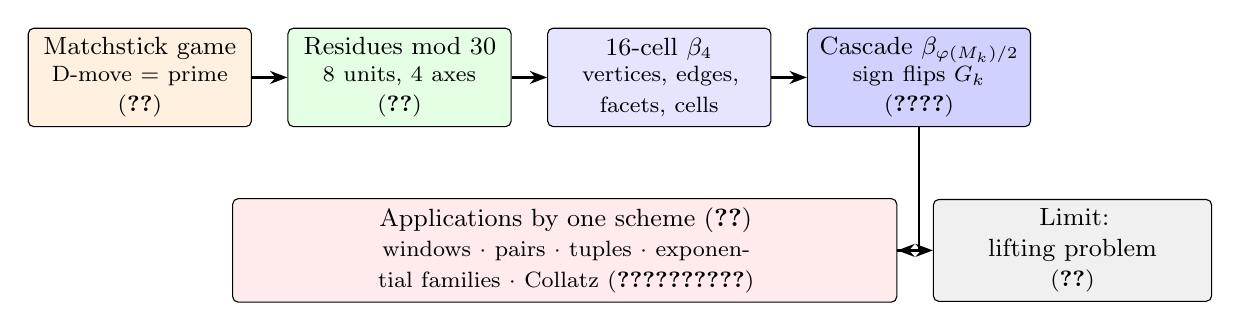
\begin{tikzpicture}[
  box/.style={draw,rounded corners=2pt,align=center,font=\small,
    minimum height=1.25cm,text width=2.6cm,fill=#1},
  box/.default=white,
  arr/.style={-{Stealth[length=2.2mm]},thick}]
\node[box=orange!12] (g) {Matchstick game\\ \footnotesize D-move $=$ prime\\\footnotesize (\cref{sec:game})};
\node[box=green!10,right=0.45cm of g] (r) {Residues mod 30\\ \footnotesize 8 units, 4 axes\\\footnotesize (\cref{sec:16cell})};
\node[box=blue!10,right=0.45cm of r] (c) {16-cell $\beta_4$\\ \footnotesize vertices, edges,\\\footnotesize facets, cells};
\node[box=blue!18,right=0.45cm of c] (k) {Cascade $\beta_{\varphi(M_k)/2}$\\ \footnotesize sign flips $G_k$\\\footnotesize (\cref{sec:cascade,sec:four})};
\node[box=red!8,below=0.9cm of c,xshift=-1.2cm,text width=8.2cm] (a) {Applications by one scheme (\cref{sec:scheme})\\
\footnotesize windows $\cdot$ pairs $\cdot$ tuples $\cdot$ exponential families $\cdot$ Collatz
 (\cref{sec:windows,sec:pairs,sec:tuples,sec:exp,sec:collatz})};
\node[box=gray!12,right=0.45cm of a,text width=3.3cm] (l) {Limit:\\ lifting problem\\\footnotesize (\cref{sec:closure})};
\draw[arr] (g)--(r); \draw[arr] (r)--(c); \draw[arr] (c)--(k);
\draw[arr] (k.south) |- (a.east);
\draw[arr] (a)--(l);
\end{tikzpicture}
\caption{Overview. The game singles out the primes; three sieve steps leave the
eight units modulo~$30$; the mirror pairing makes them the $16$-cell; the same
construction at every primorial gives a cascade on which four structural
theorems hold; one application scheme then treats the classical problems and
isolates the single step it cannot perform.}
\label{fig:overview}
\end{figure}

\paragraph{What is proved and what is not.}
All statements marked \statS\ are theorems with complete proofs. Most of them
are elementary (Chinese remainder theorem, structure of unit groups, Mertens'
theorem); their value lies in the uniform geometric organisation and in a few
sharp statements that we have not found in the literature in this form, most
notably the \emph{completeness theorem} (\cref{thm:completeness}) with its sharp
threshold $k\ge6$ (\cref{prop:sharp}). For every classical problem we separate
four layers: the exact local count (\statS), the classical conditional
asymptotic (Hardy--Littlewood type), the strongest unconditional result from
the literature, and our own numerics (\statN). The geometric constructions do
not replace the analytic input that the open problems require, and we make no
claim that they do.

\paragraph{Contributions.}
\begin{enumerate}[leftmargin=*,itemsep=1pt]
\item A self-contained account of the $16$-cell model of the units modulo $30$,
including its complete incidence spectrum (\cref{sec:16cell}).
\item A uniform treatment of the sign-flip action on $U(M_k)$: orbits are
square classes, the group is the $2$-torsion of the unit group, the Cayley
graph is a disjoint union of hypercubes, and the averaging operator has an
explicit binomial spectrum (\cref{sec:cascade,sec:four}).
\item A short rigorous proof of the completeness theorem via one divisibility
lemma ($4M_k\mid n^2-z^2$), with the sharp threshold and the identification of
$p_{k+1}^2$ as the smallest composite orbit minimum (\cref{sec:four}).
\item A six-step application scheme and its execution for the classical prime
problems, with explicit residue sets, exact counts, constants and numerics
(\cref{sec:scheme,sec:windows,sec:pairs,sec:tuples,sec:exp}).
\item A clear statement of the limit of the method (non-locality and the
lifting problem), supported by an explicit count of ``local'' versus true orbit
minima (\cref{sec:closure}).
\end{enumerate}

\paragraph{Notation.} $p_1=2,p_2=3,p_3=5,\dots$ are the primes in increasing
order, $M_k=p_1p_2\cdots p_k$ is the $k$-th primorial ($M_3=30$, $M_4=210$,
$M_5=2310$), $U(M)=(\Z/M\Z)^\times$, $\varphi$ is Euler's function, and units
modulo $M$ are represented by integers in $[1,M]$. $\beta_d$ denotes the
$d$-dimensional cross-polytope (convex hull of $\pm e_1,\dots,\pm e_d$).
A glossary for non-specialists is in \cref{app:glossary}.

% =====================================================================
\section{The matchstick game and the notion of a prime}\label{sec:game}

\begin{plainwords}
Imagine walking along the numbers $2,3,4,\dots$ and laying down one matchstick
at each number. A stick is of one of three kinds. If the number can be written
as a product of two \emph{different} smaller numbers ($12=3\cdot4$), the stick
``closes a rectangle''. If it is the square of a prime ($25=5\cdot5$), it is
an ``echo''. Otherwise nothing old explains the number, and it opens a
\emph{new direction}. The new directions are exactly the primes. Nothing deep
happens here; the game is a bookkeeping device. Its use is that it turns
multiplication into geometry: each prime is an axis, each number a point in a
lattice with one axis per prime, and many classical facts (Euler's product,
Mertens' constant, Ramanujan's highly composite numbers) become statements
about this lattice.
\end{plainwords}

\subsection{Rules}
We use the following binding formulation of the rules of \cite{K-matchstick}.
For $n\ge2$ the move at $n$ is
\begin{itemize}[itemsep=0pt]
\item \textbf{S} (\emph{closing}) if $n=ab$ with integers $1<a<b$;
\item otherwise \textbf{E} (\emph{echo}) if $n=p^2$ for a prime $p$;
\item otherwise \textbf{D} (\emph{new direction}).
\end{itemize}
The priority $S>E>D$ is part of the rule. \Cref{fig:game} shows the board for
$2\le n\le 40$.

\begin{figure}[!htbp]
\centering
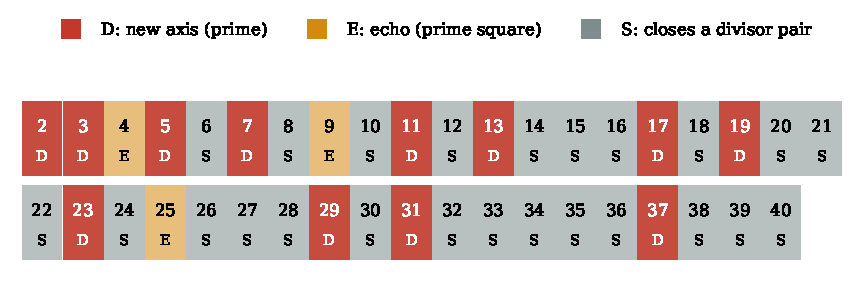
\includegraphics[width=0.92\linewidth]{figures/fig_game.pdf}
\caption{The matchstick board for $2\le n\le40$. Red: D-moves (new direction),
yellow: E-moves (prime squares $4,9,25$), grey: S-moves (closing a divisor
pair). The red cells are exactly the primes (\cref{prop:Dprime}).}
\label{fig:game}
\end{figure}

\subsection{Game primes are primes}
\begin{proposition}[\statS]\label{prop:Dprime}
For $n\ge2$ the move at $n$ is D if and only if $n$ is prime.
\end{proposition}
\begin{proof}
A prime has no factorisation $n=ab$ with $1<a\le b$, so neither S nor E
applies. Conversely let $n$ be composite with smallest prime factor $q$, and
write $n=qm$ with $m\ge q$. If $m>q$, the move is S; if $m=q$, then $n=q^2$ and
the move is E. In neither case is it D.
\end{proof}

\subsection{What the game makes visible}
\begin{plainwords}[: the lattice of exponents]
If every prime is an axis, then every number is a point whose coordinates are
its prime exponents: $12=2^2\cdot3$ sits at height $2$ on axis~$2$ and height
$1$ on axis~$3$. The total number of sticks is the number of prime factors
counted with multiplicity.
\end{plainwords}

Write $n=\prod_p p^{a_p}$. The map $n\mapsto(a_p)_p$ identifies the positive
integers with the finitely supported points of $\N_0^{\{\text{primes}\}}$;
$\Omega(n)=\sum_p a_p$ and $\omega(n)=\#\{p:a_p>0\}$ count all sticks and the
occupied axes. Three classical facts take a geometric form \statG:
\begin{enumerate}[leftmargin=*,itemsep=1pt]
\item \emph{Euler's product.} Summing $n^{-s}$ over the lattice factorises over
the axes: $\sum_{n\ge1}n^{-s}=\prod_p(1-p^{-s})^{-1}$ for $\Re s>1$.
\item \emph{Mertens.} The proportion of integers with no stick on the axes
$p\le x$ is $\prod_{p\le x}(1-1/p)\sim e^{-\gamma}/\log x$ \cite{Mertens}; this
is the density that reappears in every constant of \cref{sec:pairs,sec:tuples}.
\item \emph{Highly composite numbers.} A number $n$ is highly composite if it
has more divisors than every smaller number \cite{Ramanujan}. In the lattice
these are the points that spread their sticks most efficiently over the lowest
axes; their exponents are non-increasing in $p$. Up to $10^4$ there are $20$
of them (\cref{fig:hcn}); their distribution was determined by Nicolas
\cite{Nicolas71}, see also \cite{K-nicolas}.
\end{enumerate}
The primorials $M_k$ themselves are the ``one stick per axis'' points. A
famous criterion of Nicolas \cite{Nicolas83} states that the Riemann
hypothesis holds if and only if $M_k/\varphi(M_k)>e^\gamma\log\log M_k$ for
all $k\ge1$. We do not use this criterion, but it shows that the primorial
skeleton on which the rest of the paper is built carries deep information.

\begin{figure}[!htbp]
\centering
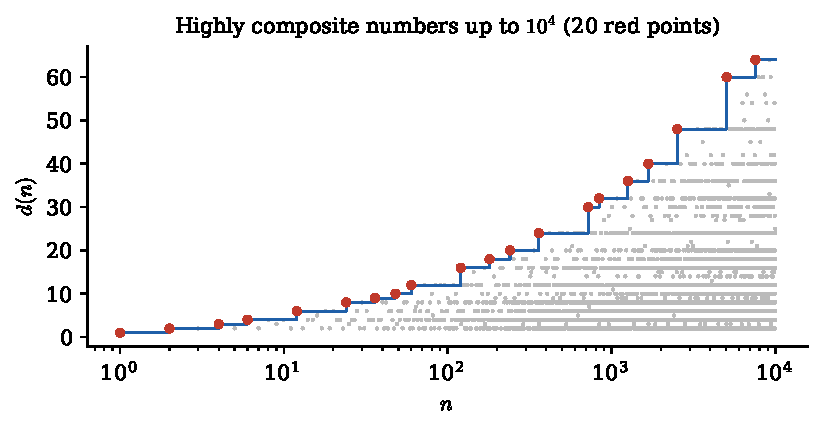
\includegraphics[width=0.62\linewidth]{figures/fig_hcn.pdf}
\caption{Divisor function $d(n)$ (grey) and the staircase of record values; the
$20$ highly composite numbers up to $10^4$ are marked red.}
\label{fig:hcn}
\end{figure}

\subsection{The adversarial version}
The \emph{Devil's game} (the sum-and-product puzzle of Freudenthal) asks for
pairs $(x,y)$ that two players can identify from the sum and the product only
after a prescribed exchange of statements. In \cite{K-devil} this puzzle is
read inside the game: every statement of the puzzle is a statement about which
factorisations of the product (S-moves) and which decompositions of the sum
remain possible, and the solutions are governed by D-moves (primes) and pure
powers of $2$. Exhaustive search finds $18$ solutions with components up to
$99\,999$ \statN\ \cite{K-devil}. We mention the puzzle only as an illustration
that ``being a D-move'' is a robust, game-theoretically usable notion; nothing
later depends on it.

% =====================================================================
\section{Residues modulo 30 and the 16-cell}\label{sec:16cell}

\begin{plainwords}
Throw away every number divisible by $2$, $3$ or $5$. What is left, modulo
$30$, are eight remainders: $1,7,11,13,17,19,23,29$. Every prime above $5$ has
one of them. These eight come in four mirror pairs that add up to $30$. Put
each pair on one axis of four-dimensional space, one remainder at $+1$ and its
mirror at $-1$, and you get eight points: the corners of the $16$-cell, the
four-dimensional analogue of the octahedron. Two corners are joined by an edge
unless they are mirror images. Edges, triangles and tetrahedra of this object
then carry arithmetic meaning: for example, the number of edges whose two
corners add up to a given remainder is exactly the local factor that appears
in the Goldbach conjecture.
\end{plainwords}

\subsection{Three sieve steps}
\begin{proposition}[\statS]
$U(30)=\{1,7,11,13,17,19,23,29\}$, $\varphi(30)=8$, and every prime $p>5$
lies in one of these classes. Moreover $U(30)\cong\Z/2\times\Z/4$: the
elements $7,13,17,23$ have order $4$, and $11,19,29$ have order $2$.
\end{proposition}
\begin{proof}
The first statement is the sieve by $2,3,5$. By the Chinese remainder theorem
$U(30)\cong U(2)\times U(3)\times U(5)\cong\Z/2\times\Z/4$. Direct computation:
$7^2=49\equiv19$, $13^2\equiv19$, $17^2\equiv19$, $23^2\equiv19$, while
$11^2\equiv19^2\equiv29^2\equiv1\pmod{30}$.
\end{proof}

\subsection{Mirror pairing and axes}
The map $a\mapsto30-a$ ($a\mapsto-a$) is a fixed-point-free involution on
$U(30)$. Its orbits are the four \emph{axes}
\[
A_1=\{1,29\},\quad A_2=\{7,23\},\quad A_3=\{11,19\},\quad A_4=\{13,17\}.
\]
\begin{definition}\label{def:16cell}
Identify the smaller element of $A_i$ with $+e_i$ and the larger with $-e_i$
in $\mathbb{R}^4$. The convex hull of these eight points is the $16$-cell
$\beta_4$. We write $A_i^+$ and $A_i^-$ for the two half-axes.
\end{definition}
In $\beta_d$ two vertices span an edge if and only if they are not antipodal;
$k+1$ vertices span a $k$-face if and only if no two are antipodal. Hence
$\beta_4$ has $f$-vector $(8,24,32,16)$: $8$ vertices, $\binom82-4=24$ edges,
$\binom43 2^3=32$ triangular facets and $2^4=16$ tetrahedral cells, each cell
choosing one vertex from every axis.

\subsection{Incidence spectrum}
\begin{proposition}[\statS]\label{prop:sums}
For the sums of vertex labels modulo $30$:
\begin{enumerate}[itemsep=0pt]
\item every axis sums to $0$;
\item the $24$ edge sums are never $0$; the classes $6,12,18,24$ occur three
times each, $10,20$ twice, and the remaining eight even classes once;
\item the $32$ facet sums are never $15$; the classes $5$ and $25$ occur four
times each, every other odd class twice;
\item the $16$ cell sums, reduced modulo $30$ and represented in $(0,30]$, take
each even value $2,4,\dots,28$ once and the value $30$ twice.
\end{enumerate}
\end{proposition}
\begin{proof}
A finite check of $4+24+32+16$ cases, reproduced in \cref{app:code}; the
distribution is shown in \cref{fig:sums}.
\end{proof}

\begin{figure}[!htbp]
\centering
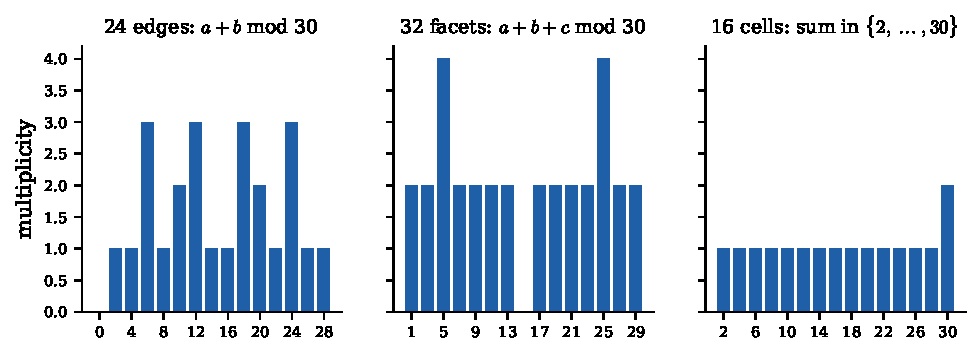
\includegraphics[width=0.92\linewidth]{figures/fig_sums.pdf}
\caption{Sum distributions of the $24$ edges, $32$ facets and $16$ cells of
the $16$-cell modulo $30$ (\cref{prop:sums}). Edge sums avoid $0$ (that is the
axis value), facet sums avoid $15$.}
\label{fig:sums}
\end{figure}

The edge spectrum is not a curiosity. For an even residue $r$ let $g_{30}(r)$
be the number of \emph{ordered} pairs $(a,b)\in U(30)^2$ with $a+b\equiv
r\pmod{30}$.

\begin{theorem}[Local Goldbach factor at 30, \statS]\label{thm:B1}
\[
g_{30}(r)=\begin{cases}8,& r\equiv0 \pmod{30},\\ 6,& 6\mid r,\ 30\nmid r,\\
4,& 10\mid r,\ 30\nmid r,\\ 3,&\text{otherwise,}\end{cases}
\qquad\text{equivalently}\qquad g_{30}(r)=\prod_{p\in\{3,5\}}N_p(r),
\]
with $N_p(r)=p-1$ if $p\mid r$ and $N_p(r)=p-2$ otherwise. Geometrically:
$g_{30}(0)=2\cdot\#\{\text{axes}\}$, and for $r\not\equiv0$,
$g_{30}(r)=2\cdot\#\{\text{edges with sum }r\}+\#\{a: 2a\equiv r\}$, the last
term being the ``diagonal'' pairs $(a,a)$.
\end{theorem}
\begin{proof}
By the Chinese remainder theorem the number of pairs factorises over $p=2,3,5$.
For $p=2$ both summands are odd, giving one pair modulo $2$ for even $r$. For
odd $p$, the pairs $(a,b)$ of non-zero residues with $a+b\equiv r$ number
$p-1$ if $r\equiv0$ (every $a\ne0$ works) and $p-2$ otherwise ($a\ne0$ and
$a\ne r$). The geometric decomposition is immediate: if $r\equiv0$ the pairs
are $(a,-a)$, i.e.\ the four axes in both orders; if $r\not\equiv0$ an
unordered pair $\{a,b\}$ with $a\ne b$ is non-antipodal, hence an edge, and
contributes two ordered pairs. Comparing with \cref{prop:sums} gives the table
(e.g.\ for $r=2$ there is the single edge $\{13,19\}$ and the diagonal pair
$(1,1)$, so $g_{30}(2)=2\cdot1+1=3$).
\end{proof}

\begin{remark}[a negative result]
The analogous attempt for sums of three units fails: the ordered triples with
sum in the odd classes $1,5,3,15$ number $39,36,26,24$, which is \emph{not}
proportional to the facet multiplicities of \cref{prop:sums}. The local factor
of the ternary Goldbach problem is still a product of local counts
(\cref{sec:pairs}), but it is not a face count of $\beta_4$.
\end{remark}

\subsection{Two great squares}
\begin{proposition}[\statS]\label{prop:G3}
The solutions of $x^2\equiv1\pmod{30}$ form the subgroup
$T_1=U(30)[2]=\{1,11,19,29\}\cong(\Z/2)^2$, and $T_2=7T_1=\{7,13,17,23\}$ is
its other coset. Geometrically $T_1=A_1\cup A_3$ and $T_2=A_2\cup A_4$ are two
orthogonal great squares of $\beta_4$ (each a $\beta_2$ lying in a coordinate
plane).
\end{proposition}
\begin{proof}
The squares were computed above. $T_1$ consists of the two axes $A_1,A_3$, so
its convex hull is the square with vertices $\pm e_1,\pm e_3$; likewise for
$T_2$.
\end{proof}
\begin{remark}
In earlier papers of the series \cite{K-16cell,K-recursive} $T_1,T_2$ were
called a ``stella octangula'' decomposition. Since each $T_i$ contains
antipodal pairs, the sets are great squares and not cells; the decomposition
is the splitting of $\mathbb{R}^4$ into two orthogonal coordinate planes.
\end{remark}

\begin{figure}[!htbp]
\centering
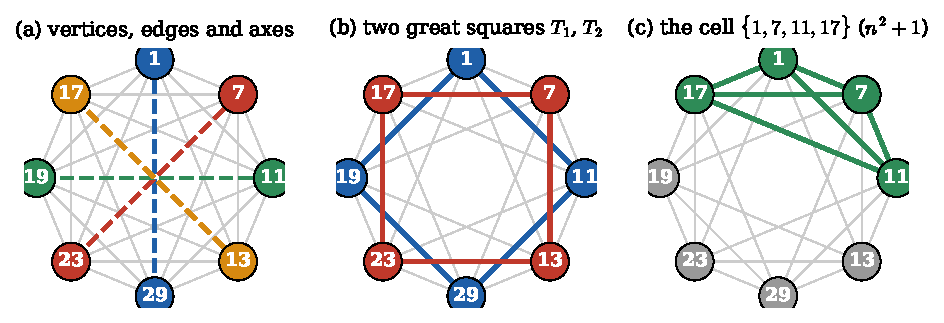
\includegraphics[width=\linewidth]{figures/fig_16cell.pdf}
\caption{The $16$-cell in the standard octagon projection. Left: the four
axes $A_1,\dots,A_4$ (dashed) and all $24$ edges. Middle: the great squares
$T_1=\{1,11,19,29\}$ (the orbit of $1$ under sign flips) and
$T_2=\{7,13,17,23\}$. Right: the cell $\{1,7,11,17\}$, which carries all primes
of the form $n^2+1$ beyond $5$ (\cref{thm:landau}).}
\label{fig:16cell}
\end{figure}

\subsection{Why the 16-cell}
There are exactly six regular convex polytopes in dimension four: the $5$-cell,
the tesseract, the $16$-cell, the $24$-cell, the $120$-cell and the $600$-cell
\cite{Coxeter}. The choice of the $16$-cell is a modelling choice, which we
state openly. It rests on three requirements: (i) eight vertices, one per unit;
(ii) a fixed-point-free central symmetry that realises $a\mapsto-a$; (iii) the
edge relation should be determined by this symmetry alone. Among the regular
four-dimensional polytopes only the $16$-cell has eight vertices, and in every
dimension the cross-polytope is the unique polytope whose graph is ``all pairs
except antipodes'' (the cocktail-party graph). For general $M_k$ the same
requirements lead to $\beta_{\varphi(M_k)/2}$ (\cref{sec:cascade}). Exploratory
checks at $210$ and $2310$ gave no indication of additional exceptional
structure (for instance root systems of type $F_4$ or $E_8$) \statN; we use
none.

\subsection{Fermat purity of 30}
\begin{proposition}[\statS]\label{prop:fermatpure}
$U(M_k)$ is a $2$-group if and only if $k\le3$. Equivalently, the
cross-polytope dimension $\varphi(M_k)/2$ is a power of two exactly for
$k\le3$, and $\varphi(M_k)/2=k+1$ holds only for $k=3$.
\end{proposition}
\begin{proof}
$|U(M_k)|=\prod_{j\le k}(p_j-1)$ is a power of $2$ iff every $p_j\le p_k$ is
of the form $2^m+1$; $2,3,5$ are, $7$ is not. The values $\varphi(M_k)/2$ are
$1,4,24,240,\dots$ for $k=2,3,4,5,\dots$ and grow faster than $k+1$.
\end{proof}
So $30$ is the last primorial whose unit group is built only from the Fermat
primes $3,5$; this is why the $16$-cell carries the clean $\Z/2\times\Z/4$
structure without odd-order components.

\subsection{The address of a prime}
\begin{definition}\label{def:address}
For a prime $p>5$ let $k$ be the smallest index with $p<M_k$. The
\emph{address} of $p$ is $(k,A_i,\pm,s)$, where $A_i^\pm$ is the half-axis
containing $p\bmod30$ and $s$ is the $0$-based position of $p$ among the
units in $[1,M_k]$ that lie on the same half-axis (there are $\varphi(M_k)/8$
such slots).
\end{definition}
Examples: $7\mapsto(3,A_2,+,0)$, $31\mapsto(4,A_1,+,1)$,
$101\mapsto(4,A_3,+,3)$. Further addresses are listed in \cref{app:tables}.
\begin{proposition}[\statS]
Distinct primes $p>5$ have distinct addresses.
\end{proposition}
\begin{proof}
The address determines $k$, the residue $p\bmod 30$ and the position among the
units below $M_k$ in that class, hence the integer $p<M_k$ itself.
\end{proof}
A second, classical label refines the half-axis \statS: a prime
$p\equiv1\pmod4$ is a sum of two squares (Fermat), $p\equiv3\pmod8$ is a sum
of three but not two squares, and $p\equiv7\pmod8$ needs four squares
(Legendre, Lagrange) \cite{HardyWright}; see \cite{K-triangle} for the square atlas. We call these the square classes
A, B, C.

% =====================================================================
\section{From 30 to every primorial: the cross-polytope cascade}\label{sec:cascade}

\begin{plainwords}
Nothing about the construction is special to $30$. Remove the multiples of
$2,3,5,7$ and you are left with $48$ remainders modulo $210$; pair them with
their mirrors and you get a $24$-dimensional cross-polytope. Each new prime
multiplies the number of corners by $p-1$. On each of these polytopes there is
a natural set of ``switches'': for every odd prime $p_j\le p_k$ one may flip
the sign of a remainder with respect to $p_j$ alone, leaving it unchanged
modulo all the other primes. Flipping all switches at once gives the mirror
image. A group of remainders that can be reached from one another by flipping
switches is called an \emph{orbit}, and its smallest member is its
\emph{orbit minimum}. Orbit minima are the central objects of the paper; the
next section shows that, in a precisely described range, they are exactly the
primes.
\end{plainwords}

\subsection{Setting}
Fix $k\ge2$. The vertex set of level $k$ is $U(M_k)$, of size
$\varphi(M_k)=\prod_{j\le k}(p_j-1)$. Because $M_k$ is even, $a\mapsto M_k-a$
is a fixed-point-free involution on $U(M_k)$ ($a=M_k/2$ is not a unit). Its
$\varphi(M_k)/2$ orbits are the \emph{axes} of level $k$, and as in
\cref{def:16cell} the units become the vertices of $\beta_{\varphi(M_k)/2}$.

\subsection{Sign-flip action}
For $2\le j\le k$ let $e_j\in U(M_k)$ be the unique unit with
$e_j\equiv-1\pmod{p_j}$ and $e_j\equiv1\pmod{p_i}$ for $i\ne j$, and define
$\sigma_j(a)=e_ja\bmod M_k$. Thus $\sigma_j$ flips the sign of $a$ modulo
$p_j$ and changes nothing else. Let $G_k=\langle\sigma_2,\dots,\sigma_k\rangle$.

\begin{proposition}[\statS]\label{prop:Gk}
\begin{enumerate}[itemsep=0pt]
\item $G_k\cong(\Z/2)^{k-1}$, and $G_k$ acts on $U(M_k)$ by multiplication
with the subgroup $U(M_k)[2]=\{x:x^2\equiv1\}=\{\prod_{j\in S}e_j:S\subseteq\{2,\dots,k\}\}$.
\item The action is free.
\item The product of all $\sigma_j$ is the antipodal map $a\mapsto-a$.
\end{enumerate}
\end{proposition}
\begin{proof}
By the Chinese remainder theorem $U(M_k)\cong\prod_{j\le k}U(p_j)$, and for
odd $p_j$ the cyclic group $U(p_j)$ has $2$-torsion $\{\pm1\}$, while $U(2)$ is
trivial. Hence $U(M_k)[2]\cong(\Z/2)^{k-1}$ with basis $e_2,\dots,e_k$. A
multiplication by a group element $g\ne1$ has no fixed point, so the action is
free. Finally $\prod_je_j\equiv-1$ modulo every odd $p_j$ and modulo $2$.
\end{proof}

\subsection{Orbit criterion}
\begin{proposition}[\statS]\label{prop:orbitcrit}
Two units $y,z$ lie in the same $G_k$-orbit if and only if
$y^2\equiv z^2\pmod{M_k}$, equivalently $z\equiv\pm y\pmod{p_j}$ for every odd
$p_j\le p_k$. Every orbit is a union of $2^{k-2}$ axes.
\end{proposition}
\begin{proof}
$z\in yU(M_k)[2]$ iff $(z/y)^2\equiv1$ iff $z^2\equiv y^2$. Modulo an odd
prime, $z^2\equiv y^2$ means $z\equiv\pm y$. By \cref{prop:Gk}(3) every orbit
is closed under $a\mapsto-a$; it has $2^{k-1}$ elements, hence $2^{k-2}$ axes.
\end{proof}

\subsection{Counting}
\begin{definition}
$B_k$ is the set of orbit minima, i.e.\ the smallest representative in
$[1,M_k]$ of every $G_k$-orbit.
\end{definition}
\begin{corollary}[\statS]\label{cor:count}
$|B_k|=\varphi(M_k)/2^{k-1}$, and every orbit minimum is $<M_k/2$. Explicitly
$|B_k|=2,6,30,180,1440,12960$ for $k=3,\dots,8$.
\end{corollary}
\begin{proof}
The action is free, so all orbits have $2^{k-1}$ elements. An orbit contains
$y$ and $M_k-y$, and one of them is $<M_k/2$.
\end{proof}

\begin{figure}[!htbp]
\centering
\begin{minipage}{0.56\linewidth}\centering
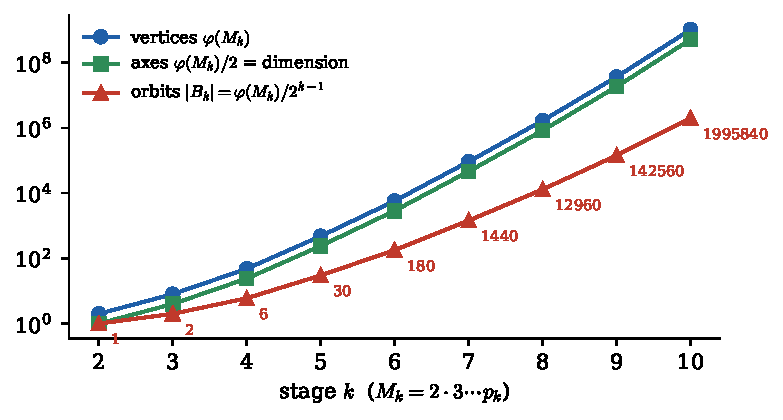
\includegraphics[width=\linewidth]{figures/fig_cascade.pdf}
\end{minipage}\hfill
\begin{minipage}{0.42\linewidth}\centering
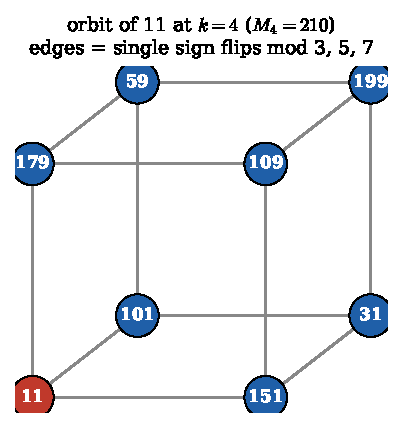
\includegraphics[width=\linewidth]{figures/fig_orbitcube.pdf}
\end{minipage}
\caption{Left: growth of the cascade. Vertices $\varphi(M_k)$, cross-polytope
dimension $\varphi(M_k)/2$ and number of orbits $|B_k|$ on a logarithmic scale.
Right: the orbit of $11$ modulo $210$ drawn as the cube $Q_3$; each edge
direction is one sign flip $\sigma_2,\sigma_3,\sigma_4$ (modulo $3,5,7$), and
the orbit minimum $11$ is marked red.}
\label{fig:cascade}
\end{figure}

% =====================================================================
\section{Four structural theorems}\label{sec:four}

\begin{plainwords}
Four facts organise the cascade. \emph{Symmetry}: two remainders are in the
same orbit exactly when their squares agree; the mirror is one of the
switches. \emph{Completeness}: from level $k=6$ on (modulus $30030$), every
orbit minimum up to the square of the next prime is a prime, and every prime in
that range is an orbit minimum, with exactly one exception, the square
$p_{k+1}^2$ itself. Below level $6$ this is false, and we show exactly where it
fails. \emph{Recursion}: the next prime is always the smallest orbit minimum
larger than $1$; so the machine ``knows'' the next prime. \emph{Growth}: each
new level multiplies the number of orbits by $(p-1)/2$. The heart of the proof
of completeness is a single observation: two different numbers in the same
orbit must have squares that differ by a multiple of $4M_k$, which is
impossible if both are small.
\end{plainwords}

\begin{figure}[!htbp]
\centering
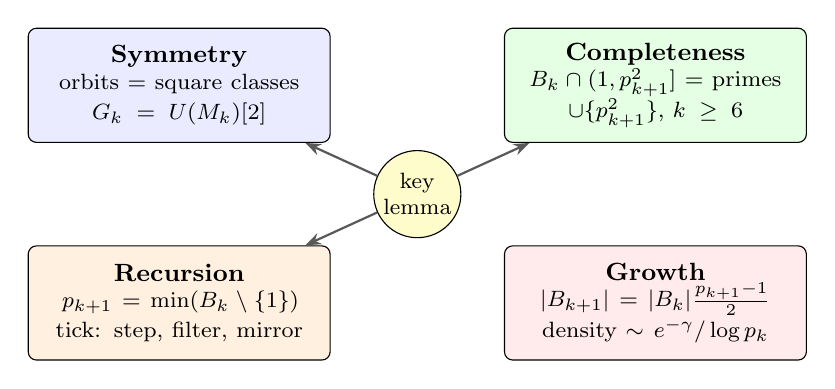
\begin{tikzpicture}[
  th/.style={draw,rounded corners=3pt,align=center,font=\small,
    minimum height=1.45cm,text width=3.6cm,fill=#1},
  arr/.style={-{Stealth[length=2mm]},thick,gray!70!black}]
\node[th=blue!8] (s) {\textbf{Symmetry}\\\footnotesize orbits $=$ square classes\\\footnotesize $G_k=U(M_k)[2]$};
\node[th=green!10,right=2.2cm of s] (c) {\textbf{Completeness}\\\footnotesize $B_k\cap(1,p_{k+1}^2]$ $=$ primes\\\footnotesize $\cup\{p_{k+1}^2\}$, $k\ge6$};
\node[th=orange!12,below=1.3cm of s] (r) {\textbf{Recursion}\\\footnotesize $p_{k+1}=\min(B_k\setminus\{1\})$\\\footnotesize tick: step, filter, mirror};
\node[th=red!8,below=1.3cm of c] (g) {\textbf{Growth}\\\footnotesize $|B_{k+1}|=|B_k|\tfrac{p_{k+1}-1}{2}$\\\footnotesize density $\sim e^{-\gamma}/\log p_k$};
\node[draw,circle,fill=yellow!20,font=\footnotesize,align=center,inner sep=1pt] at ($(s)!0.5!(g)$) (k) {key\\lemma};
\draw[arr] (k)--(s); \draw[arr] (k)--(c); \draw[arr] (k)--(r); 
\end{tikzpicture}
\caption{The four structural theorems. The key lemma
(\cref{lem:key}: $z\sim n\Rightarrow 4M_k\mid n^2-z^2$) drives completeness and
recursion; symmetry provides the orbit criterion on which everything rests.}
\label{fig:four}
\end{figure}

\subsection{Symmetry}
\begin{theorem}[Symmetry, \statS]\label{thm:symmetry}
The $G_k$-orbits on $U(M_k)$ are the fibres of the squaring map
$U(M_k)\to U(M_k)^2$; $G_k$ is the $2$-torsion subgroup $U(M_k)[2]$; the
antipodal map is the all-flip element. In particular $B_k$ is in bijection with
the group of squares $U(M_k)^2$, and $|U(M_k)^2|=\varphi(M_k)/2^{k-1}$.
\end{theorem}
\begin{proof}
This is \cref{prop:Gk,prop:orbitcrit,cor:count} combined.
\end{proof}

\subsection{Completeness}
\begin{lemma}[Key lemma, \statS]\label{lem:key}
Let $k\ge2$ and let $z<n$ be units in the same $G_k$-orbit. Then
$4M_k\mid n^2-z^2$. Consequently every unit $n$ with $n^2\le4M_k$ is an
orbit minimum.
\end{lemma}
\begin{proof}
By \cref{prop:orbitcrit} every odd $p_j\le p_k$ divides $n^2-z^2$, so
$M_k/2\mid n^2-z^2$. Both $n,z$ are odd, and the square of an odd number is
$\equiv1\pmod8$, so $8\mid n^2-z^2$. As $M_k/2$ is odd, $4M_k=8\cdot M_k/2$
divides $n^2-z^2$. If $n^2\le4M_k$ and some $z<n$ lay in the orbit of $n$, then
$0<n^2-z^2<n^2\le4M_k$, a contradiction.
\end{proof}

\begin{lemma}[\statS]\label{lem:units}
Every unit $n$ modulo $M_k$ with $1<n\le p_{k+1}^2$ is either a prime in
$(p_k,p_{k+1}^2)$ or equal to $p_{k+1}^2$.
\end{lemma}
\begin{proof}
All prime factors of $n$ are $\ge p_{k+1}$. If $n$ has at least two of them
(with multiplicity), then $n\ge p_{k+1}^2$, hence $n=p_{k+1}^2$.
\end{proof}

\begin{lemma}[\statS]\label{lem:threshold}
$4M_k\ge p_{k+1}^4$ holds if and only if $k\ge6$.
\end{lemma}
\begin{proof}
For $k=1,\dots,5$ the pairs $(4M_k,p_{k+1}^4)$ are $(8,81)$, $(24,625)$,
$(120,2401)$, $(840,14641)$, $(9240,28561)$. For $k=6$:
$4M_6=120120\ge17^4=83521$. If $4M_k\ge p_{k+1}^4$ for some $k\ge6$, then by
Bertrand's postulate $p_{k+2}<2p_{k+1}$, so
$p_{k+2}^4<16\,p_{k+1}^4\le p_{k+1}\cdot p_{k+1}^4\le p_{k+1}\cdot4M_k=4M_{k+1}$,
using $p_{k+1}\ge17>16$.
\end{proof}

\begin{theorem}[Completeness, \statS]\label{thm:completeness}
For every $k\ge6$,
\[
B_k\cap(1,p_{k+1}^2]\;=\;\{\,p\text{ prime}: p_k<p<p_{k+1}^2\,\}\;\cup\;\{p_{k+1}^2\}.
\]
In particular the orbit minima in the window $I_k=(p_k,p_k^2]$ are exactly the
primes in $I_k$, and $p_{k+1}^2$ is the smallest composite orbit minimum
($289,361,529$ for $k=6,7,8$).
\end{theorem}
\begin{proof}
Orbit minima are units, so by \cref{lem:units} the left side is contained in
the right side. Conversely every element $n$ of the right side is a unit with
$n\le p_{k+1}^2\le2\sqrt{M_k}$ by \cref{lem:threshold}, hence $n^2\le4M_k$, and
$n$ is an orbit minimum by \cref{lem:key}. Since $p_k^2<p_{k+1}^2$, the window
statement follows.
\end{proof}

\begin{proposition}[Sharpness, \statS]\label{prop:sharp}
The window statement fails for $k=3,4,5$. At $k=5$ ($M_5=2310$,
$2\sqrt{M_5}\approx96.1$) all primes in $(11,96]$ are orbit minima, but the
four primes $97,101,103,107$ are not: they lie in the orbits of
$13,31,37,47$, respectively, with $n^2-z^2=4M_5$ in each case (e.g.\
$97^2-13^2=9240$). At $k=4$, $31^2-11^2=840=4M_4$; at $k=3$, $B_3=\{1,7\}$.
The smallest composite orbit minimum at $k=5$ is $247=13\cdot19$.
\end{proposition}
\begin{proof}
Direct verification with the orbit criterion; the code is in \cref{app:code}.
\end{proof}

\begin{figure}[!htbp]
\centering
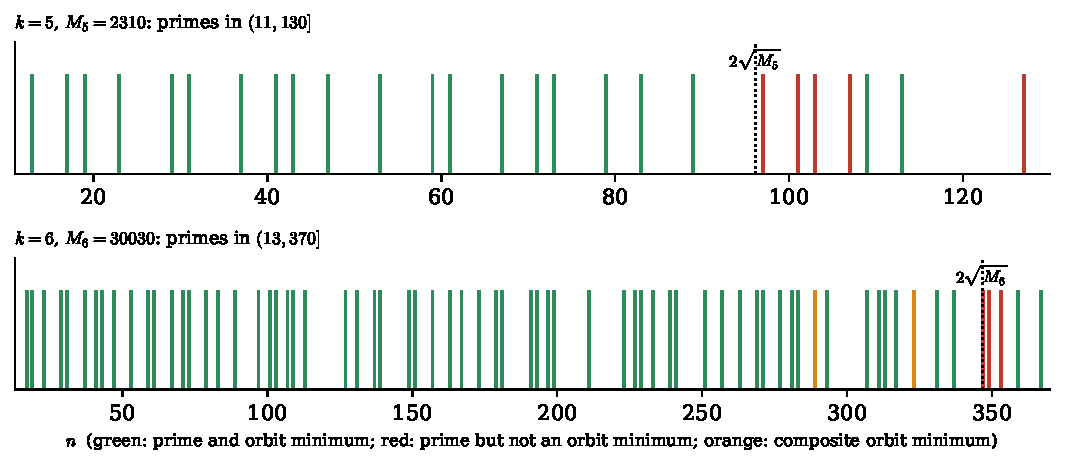
\includegraphics[width=0.95\linewidth]{figures/fig_threshold.pdf}
\caption{The threshold $2\sqrt{M_k}$ of the key lemma. Top ($k=5$): primes up
to $2\sqrt{M_5}\approx96.1$ are orbit minima (green), the four primes
$97$--$107$ are not (red). Bottom ($k=6$): every prime up to $2\sqrt{M_6}\approx
346.6$ is an orbit minimum; the first composite orbit minimum is $17^2=289$
(orange), as predicted by \cref{thm:completeness}.}
\label{fig:threshold}
\end{figure}

\begin{remark}[what completeness does and does not say]
\Cref{thm:completeness} is a \emph{characterisation}, not an existence theorem
for primes: it says that the orbit-minimum construction, applied in its
window, produces the primes and nothing else. It does not by itself imply
that the window contains a prime; that follows from Bertrand's postulate
(\cref{sec:windows}). At $k=6$ there are $27$ composite orbit minima below
$M_6/2$; above $p_{k+1}^2$ composites appear and their share grows with $n$.
\end{remark}

\subsection{Self-similarity and recursion}
\begin{theorem}[Recursion, \statS]\label{thm:recursion}
\begin{enumerate}[itemsep=0pt]
\item For every $k\ge3$, $p_{k+1}=\min(B_k\setminus\{1\})$.
\item Reduction modulo $M_k$ maps every $G_{k+1}$-orbit onto a $G_k$-orbit, and
over every $G_k$-orbit lie exactly $(p_{k+1}-1)/2$ orbits of level $k+1$. Hence
$|B_{k+1}|=|B_k|\,(p_{k+1}-1)/2$.
\end{enumerate}
\end{theorem}
\begin{proof}
(1) $p_{k+1}$ is the smallest unit $>1$. By Bertrand $p_{k+1}<2p_k$, and
$p_k^2\le M_k$ for $k\ge3$ (since $M_{k-1}\ge2p_{k-1}>p_k$), so
$p_{k+1}^2<4p_k^2\le4M_k$, and $p_{k+1}$ is an orbit minimum by
\cref{lem:key}. No unit strictly between $1$ and $p_{k+1}$ exists.
(2) By the Chinese remainder theorem the square map factorises:
$y^2\bmod M_{k+1}\leftrightarrow(y^2\bmod M_k,\ y^2\bmod p_{k+1})$. Orbits of
level $k+1$ are therefore pairs (orbit of level $k$, non-zero square class
modulo $p_{k+1}$), and $U(p_{k+1})$ has $(p_{k+1}-1)/2$ squares.
\end{proof}
The passage $k\to k+1$ is the \emph{tick} of the machine \cite{K-recursive}:
\emph{step} (multiply the modulus by $p_{k+1}$), \emph{filter} (remove the
multiples of $p_{k+1}$, so $|U|$ is multiplied by $p_{k+1}-1$) and
\emph{mirror} (adjoin the new sign flip $\sigma_{k+1}$, so $|G|$ doubles).

\subsection{Convergence and branching}
\begin{proposition}[\statS]
The vertex density of level $k$ is
$\varphi(M_k)/M_k=\prod_{p\le p_k}(1-1/p)\sim e^{-\gamma}/\log p_k$ (Mertens),
the branching factor of vertices is $p_{k+1}-1$, and that of orbits is
$(p_{k+1}-1)/2$.
\end{proposition}
The density is the probability that a random integer survives the sieve up to
$p_k$. Near $x=p_k^2$ the survivors of the sieve up to $\sqrt x$ are exactly the
primes, yet the sieve density there is $2e^{-\gamma}/\log x\approx1.123/\log x$,
not the prime density $1/\log x$. This classical mismatch (Mertens' constant
$e^{-\gamma}$ instead of $1/2$) shows that local sieve counts do not
automatically become prime counts; it is the simplest instance of the gap
between steps~4 and~5 of the scheme in \cref{sec:scheme}.

\subsection{Cross-check in four languages}
\begin{plainwords}[: four ways to see the same object]
The same orbit structure can be described in four mathematical languages:
as a graph (each orbit is a hypercube), as a linear operator (an averaging
operator with a simple spectrum), as a table of quadratic residues (Legendre
symbols), and as a growth law. They all say the same thing, which is a useful
consistency check and makes the construction accessible from several fields \cite{K-layers}.
\end{plainwords}

\begin{proposition}[\statS]\label{prop:languages}
\begin{enumerate}[itemsep=1pt]
\item \emph{Graph.} The Cayley graph of the action (generators
$\sigma_2,\dots,\sigma_k$) is a disjoint union of $|B_k|$ copies of the
hypercube $Q_{k-1}$.
\item \emph{Operator.} Let $U_j$ be the permutation operator of $\sigma_j$ on
functions $U(M_k)\to\mathbb{C}$ and $T=\frac1k\bigl(I+\sum_{j=2}^kU_j\bigr)$.
The eigenvalues of $T$ are $(k-2m)/k$, $m=0,\dots,k-1$, with multiplicity
$|B_k|\binom{k-1}{m}$.
\item \emph{Legendre.} For an odd prime $p_i\ne p_j$ the Legendre symbol
$(\sigma_j a/p_i)=(a/p_i)$, while $(\sigma_j a/p_j)=(-1/p_j)(a/p_j)$; thus
$\sigma_j$ flips the quadratic character modulo $p_j$ if and only if
$p_j\equiv3\pmod4$.
\item \emph{Growth.} $|B_{k+1}|/|B_k|=(p_{k+1}-1)/2$ (\cref{thm:recursion}).
\end{enumerate}
\end{proposition}
\begin{proof}
(1) A free action of $(\Z/2)^{k-1}$ with its standard generators makes each
orbit a copy of the Cayley graph of $(\Z/2)^{k-1}$, which is $Q_{k-1}$.
(2) On each orbit $T$ acts as $\frac1k(1+\sum_j g_j)$ in the regular
representation of $(\Z/2)^{k-1}$; on the character $\chi_S$
($S\subseteq\{2,\dots,k\}$, $|S|=m$) it has the eigenvalue
$\frac1k(1+(k-1-m)-m)$. (3) $\sigma_ja\equiv a\pmod{p_i}$ and $\equiv-a\pmod{p_j}$,
and $(-1/p)=(-1)^{(p-1)/2}$.
\end{proof}

\begin{observation}[non-locality, \statN]\label{obs:nonlocal}
Call a unit a \emph{local minimum} if it is smaller than each of its $k-1$
single-flip neighbours $\sigma_j(a)$. Every orbit minimum is a local minimum,
but the converse fails from $k=4$ on:
\begin{center}
\begin{tabular}{lrrrrrr}\toprule
$k$ & 3 & 4 & 5 & 6 & 7 & 8\\\midrule
local minima & 2 & 18 & 130 & 1263 & 18328 & 293743\\
orbit minima $|B_k|$ & 2 & 6 & 30 & 180 & 1440 & 12960\\\bottomrule
\end{tabular}
\end{center}
Being an orbit minimum is therefore a genuinely global property of the
hypercube $Q_{k-1}$; it cannot be tested by looking at neighbours only. This is
the first appearance of the non-locality that limits the method
(\cref{sec:closure}).
\end{observation}

\subsection{Algorithmic position}
Completeness yields an algorithm that lists the primes in $(p_k,p_{k+1}^2)$ in
increasing order as orbit minima \cite{K-tool}. Its cost is that of a wheel
sieve with wheel $M_k$; it is a transparent reference implementation, not a
competitor of optimised segmented sieves such as \texttt{primesieve}
\statN. We use it only as an independent check of the theory.

% =====================================================================
\section{The application scheme}\label{sec:scheme}

\begin{plainwords}
All classical questions about primes in patterns (twins, Goldbach pairs,
prime triplets, \dots) are treated by the same recipe. First, translate the
pattern into a configuration on the polytope: twin primes are pairs of corners
that differ by $2$, Goldbach pairs are corners that add up to $N$. Second,
determine on which half-axes such a configuration can live at all. Third,
count exactly how many admissible configurations exist at level $k$; this is
pure counting with the Chinese remainder theorem. Fourth, turn the count into
a density; as $k$ grows, it converges to the famous constant in the
Hardy--Littlewood prediction. Fifth comes the step the geometry cannot do:
show that the admissible configurations are really occupied by primes,
infinitely often. We call this the \emph{lifting problem}; for each problem we
state what is known classically. Sixth, we compare the predictions with
counts up to $10^8$.
\end{plainwords}

\begin{figure}[!htbp]
\centering
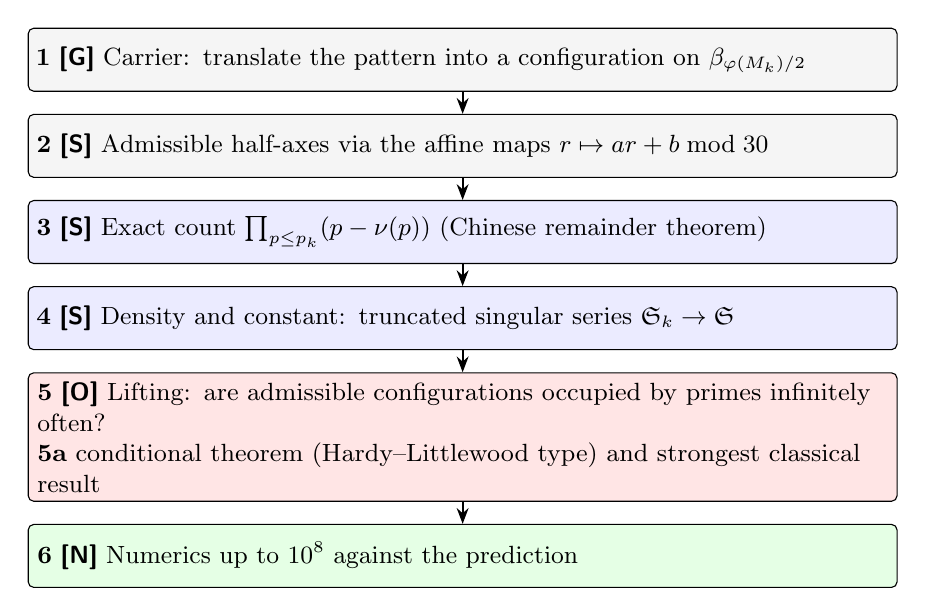
\begin{tikzpicture}[node distance=0.28cm,
  st/.style={draw,rounded corners=2pt,font=\small,align=left,text width=10.8cm,
    minimum height=0.8cm,fill=#1},
  arr/.style={-{Stealth[length=2mm]},thick}]
\node[st=gray!8] (1) {\textbf{1} \statG\ Carrier: translate the pattern into a configuration on $\beta_{\varphi(M_k)/2}$};
\node[st=gray!8,below=of 1] (2) {\textbf{2} \statS\ Admissible half-axes via the affine maps $r\mapsto ar+b \bmod 30$};
\node[st=blue!8,below=of 2] (3) {\textbf{3} \statS\ Exact count $\prod_{p\le p_k}(p-\nu(p))$ (Chinese remainder theorem)};
\node[st=blue!8,below=of 3] (4) {\textbf{4} \statS\ Density and constant: truncated singular series $\mathfrak S_k\to\mathfrak S$};
\node[st=red!10,below=of 4] (5) {\textbf{5} \statO\ Lifting: are admissible configurations occupied by primes infinitely often?\\
\textbf{5a} conditional theorem (Hardy--Littlewood type) and strongest classical result};
\node[st=green!10,below=of 5] (6) {\textbf{6} \statN\ Numerics up to $10^8$ against the prediction};
\foreach \a/\b in {1/2,2/3,3/4,4/5,5/6} \draw[arr] (\a)--(\b);
\end{tikzpicture}
\caption{The application scheme. Steps 1--4 are exact; step~5 is where the
classical difficulty sits; step~6 is the empirical check.}
\label{fig:scheme}
\end{figure}

\subsection{Admissible patterns and the exact count}
A finite set $H=\{h_1,\dots,h_m\}\subset\Z$ (a \emph{pattern}) is
\emph{admissible} if for every prime $p$ the set $H\bmod p$ misses at least one
residue class. Write $\nu_H(p)=\#(H\bmod p)$.

\begin{proposition}[Exact count, \statS]\label{prop:crt}
The number of $a\in\Z/M_k$ such that $a+h$ is a unit for every $h\in H$ is
\[
N_k(H)=\prod_{p\le p_k}\bigl(p-\nu_H(p)\bigr).
\]
\end{proposition}
\begin{proof}
By the Chinese remainder theorem the condition splits into independent
conditions modulo each $p\le p_k$, and modulo $p$ the admissible $a$ are those
avoiding the $\nu_H(p)$ classes $-h\bmod p$.
\end{proof}

\begin{proposition}[Truncated singular series, \statS]\label{prop:singular}
Define $\mathfrak S_k(H)=N_k(H)\,M_k^{m-1}/\varphi(M_k)^m$. Then
\[
\mathfrak S_k(H)=\prod_{p\le p_k}\Bigl(1-\frac{\nu_H(p)}{p}\Bigr)\Bigl(1-\frac1p\Bigr)^{-m}
\;\xrightarrow[k\to\infty]{}\;\mathfrak S(H),
\]
the Hardy--Littlewood singular series of $H$ \cite{HL}, and the product converges
absolutely. $\mathfrak S(H)>0$ if and only if $H$ is admissible.
\end{proposition}
\begin{proof}
The identity is \cref{prop:crt} divided by $M_k\prod_p(1-1/p)^m$. For $p$
larger than all differences $h_i-h_j$, $\nu_H(p)=m$ and the factor is
$1-\binom m2p^{-2}+O(p^{-3})$, so the product converges absolutely; it vanishes
iff some factor vanishes, i.e.\ iff $\nu_H(p)=p$ for some $p$.
\end{proof}

\begin{reading}[\statG]
$N_k(H)$ is the number of placements of the pattern $H$ on the vertices of
$\beta_{\varphi(M_k)/2}$, and $\mathfrak S_k(H)$ compares it with $m$
independent random vertices. The Hardy--Littlewood constant is thus the
limit of an exact vertex count on the cascade.
\end{reading}

\subsection{Three classes of prime families}
The atlas of prime families \cite{K-atlas} sorts the classical families into
three heuristic growth classes \statH:
\emph{Class 1a} (pairs and tuples with a polynomial relation: twins, cousins,
sexy primes, Sophie Germain primes): count $\sim c\,x/\log^mx$ with $c$ a
singular series;
\emph{AP-factor class} (Mersenne, Fermat, repunit, Cullen, Woodall, Proth):
divisibility forces every prime factor onto a progression of small density,
and the expected count grows like $c\log x$;
\emph{Class 3} (self-correlation conditions modulo $p^2$: Wieferich, Wilson,
Wall--Sun--Sun, Wolstenholme): expected count $\sim c\log\log x$ from the
divergence of $\sum1/p$.
\Cref{sec:pairs,sec:tuples} treat Class~1a, \cref{sec:exp} the other two.

% =====================================================================
\section{Applications I: windows and completeness}\label{sec:windows}

\begin{plainwords}
The completeness theorem says that, in a window between a prime and the square
of the next prime, the orbit minima are exactly the primes. Several old
questions ask whether such windows, or smaller ones, always contain primes.
For the window from $n$ to $2n$ the answer is yes (Bertrand's postulate, proved
in 1852). For the gaps between consecutive squares (Legendre, Brocard) the
answer is not known. The geometry turns these questions into exact statements
about how many orbit minima lie in a given range, but it does not supply the
missing analytic estimate.
\end{plainwords}

\subsection{Bertrand}
\begin{theorem}[Chebyshev; Erd\H{o}s' proof \cite{Erdos32}, \statS]
For every $n\ge1$ there is a prime $p$ with $n<p\le2n$.
\end{theorem}
Erd\H{o}s' proof compares the size of the central binomial coefficient
$\binom{2n}n\ge4^n/(2n+1)$ with the product of its prime-power factors: if
$(n,2n]$ contained no prime, every prime factor would be $\le2n/3$, which forces
$\binom{2n}n\le(2n)^{\sqrt{2n}}\,4^{2n/3}$, impossible for large $n$; small $n$
are checked directly. In \cite{K-bertrand} this argument is read as a balance
on ``Pascal's dome'' \statG. In the cascade, Bertrand guarantees the ladder
$p_k<p_{k+1}<2p_k$, i.e.\ the step of every tick lands in the window $I_k$,
and it is the only analytic input used in \cref{lem:threshold,thm:recursion}.

\subsection{Brocard}
\begin{reading}[\statG]\label{read:brocard}
For $k\ge6$, \cref{thm:completeness} gives
\[
\#\{\text{primes in }(p_k^2,p_{k+1}^2)\}=\#\bigl(B_k\cap(p_k^2,p_{k+1}^2)\bigr).
\]
Brocard's conjecture (at least four primes between $p_k^2$ and $p_{k+1}^2$ for
$k\ge2$) is therefore equivalent, for $k\ge6$, to the statement that the upper
part $(p_k^2,p_{k+1}^2)$ of the completeness range always contains at least four
orbit minima.
\end{reading}
\begin{observation}[\statN]
For $k=2,\dots,15$ the number of primes in $(p_k^2,p_{k+1}^2)$ is
$5,6,15,9,22,11,27,47,16,57,44,20,46,80$. The conjecture is open \statO.
\end{observation}

\subsection{Legendre, Andrica, Oppermann}
Legendre's conjecture (a prime between $n^2$ and $(n+1)^2$), Andrica's
conjecture ($\sqrt{p_{n+1}}-\sqrt{p_n}<1$) and Oppermann's conjecture (primes
in $(n^2-n,n^2)$ and $(n^2,n^2+n)$) are all open \statO. Each would follow from
a gap bound $p_{n+1}-p_n\ll p_n^{1/2-\varepsilon}$. The best unconditional
exponent is $0.525$ (Baker--Harman--Pintz \cite{BHP}); between consecutive
\emph{cubes} there is a prime for all large $n$ (Ingham \cite{Ingham}). In the
geometry all three statements are window statements of the type of
\cref{read:brocard} \statG; the method gives the exact count of candidates
(units) in every window, but no lower bound for the primes among them.

\subsection{Fermat numbers}
\begin{proposition}[\statS]\label{prop:fermat}
For $n\ge2$ the Fermat number $F_n=2^{2^n}+1$ satisfies $F_n\equiv17\pmod{30}$;
it lies on the half-axis $A_4^-$. Every prime factor $q$ of $F_n$ satisfies
$q\equiv1\pmod{2^{n+2}}$.
\end{proposition}
\begin{proof}
$2^{2^n}\equiv1\pmod3$ (even exponent) and $\pmod5$ (exponent divisible by $4$),
so $F_n\equiv2\pmod{15}$, and $F_n$ is odd. The divisor statement is the
classical theorem of Euler and Lucas \cite{HardyWright}.
\end{proof}
Since $\sum_n1/\log F_n$ converges, the probabilistic heuristic predicts only
finitely many Fermat primes \statH\ \cite{HardyWright}; whether there is a
Fermat prime beyond $F_4=65537$ is open \statO. In \cite{K-fermat} the
heuristic is read as a statement about the shrinking share of the
progression $1\bmod2^{n+2}$ on the cascade \statG. Note the coincidence with
\cref{prop:fermatpure}: $30$ is built only from Fermat primes, and every $F_n$
($n\ge2$) sits on one fixed half-axis of its $16$-cell.

% =====================================================================
\section{Applications II: pairs (translation and antipode)}\label{sec:pairs}

\begin{plainwords}
There are two basic ways in which two corners of the polytope can be related.
They can differ by a fixed amount (a \emph{translation}): twin primes differ by
$2$, ``sexy'' primes by $6$. Or they can add up to a fixed amount (an
\emph{antipode}, generalised): a Goldbach pair adds up to $N$. In both cases
the polytope tells us exactly on which corners such pairs can sit and how many
admissible pairs there are at each level. The count explains, for instance,
why even numbers divisible by $30$ have about $8/3$ times as many Goldbach
representations as numbers like $2\cdot7$: the factor $8/3$ is the number of
the ratio $8:3$ of the ordered pair counts for axes and for edges plus diagonal in
\cref{thm:B1}.
\end{plainwords}

\subsection{Twin primes}
\begin{theorem}[\statS]\label{thm:twin}
\begin{enumerate}[itemsep=0pt]
\item The lower member $p>5$ of a twin pair lies in one of the classes
$\{11,17,29\}\pmod{30}$; the pair $\{p,p+2\}$ is always an edge (never an axis)
of every $\beta_{\varphi(M_k)/2}$.
\item The number of twin configurations at level $k$ is
$N_k(\{0,2\})=\prod_{3\le p\le p_k}(p-2)$, i.e.\ $1$, $3$, $15$, $135$, $1485$, $22275$ for
$k=2,\dots,7$.
\item The renormalised edge density
$\delta_k=N_k(\{0,2\})/\varphi(M_k)$ satisfies
\[\frac{\delta_k\log p_k}{2e^{-\gamma}}\;\longrightarrow\;C_2=\prod_{p\ge3}\Bigl(1-\frac1{(p-1)^{2}}\Bigr)=0.6601618\ldots\]
\end{enumerate}
\end{theorem}
\begin{proof}
(1) $r$ and $r+2$ must both be units modulo $30$. A pair $\{a,a+2\}$ is an axis
iff $2a+2\equiv0\pmod{M_k}$, i.e.\ $a\equiv M_k/2-1$, which is even and hence
not a unit. (2) is \cref{prop:crt}. (3)
$(p-2)/(p-1)=\frac{p(p-2)}{(p-1)^2}\cdot\frac{p-1}p$, hence
$\delta_k=C_2^{(k)}\cdot2\prod_{p\le p_k}(1-1/p)$ with the partial product
$C_2^{(k)}\to C_2$, and Mertens' theorem gives the limit.
\end{proof}
The convergence in (3) is slow but monotone in tendency: the renormalised
density is $0.5375$ at $k=3$, $0.5889$ at $k=6$, $0.6301$ at $k=10$ and
$0.6497$ at $k=39$ \statN\ (\cref{fig:twin}); see \cite{K-c2,K-twin}.

\begin{figure}[!htbp]
\centering
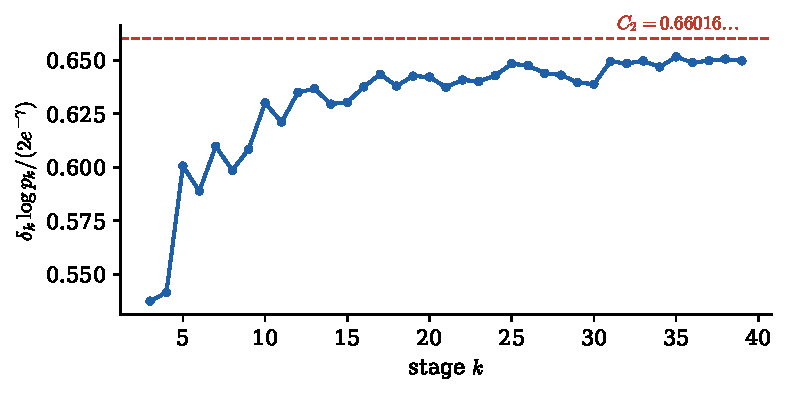
\includegraphics[width=0.62\linewidth]{figures/fig_twin.pdf}
\caption{Renormalised twin-edge density $\delta_k\log p_k/(2e^{-\gamma})$ for
$k=3,\dots,39$ and its limit $C_2$ (\cref{thm:twin}).}
\label{fig:twin}
\end{figure}

\begin{conditional}[Hardy--Littlewood \cite{HL}]
If the prime pair conjecture holds for $H=\{0,2\}$, then
$\pi_2(x)=\#\{p\le x:p+2\text{ prime}\}\sim2C_2\Li_2(x)$, with
$\Li_m(x)=\int_2^x\mathrm dt/\log^mt$.
\end{conditional}
\paragraph{Classical anchor.} Infinitely many primes $p$ with $p+2$ having at most
two prime factors (Chen \cite{Chen}); infinitely many prime gaps $\le246$
(Zhang \cite{Zhang}, Maynard \cite{Maynard}, Polymath \cite{Polymath}). In the
language of the cascade: \emph{some} admissible edge pattern of length $\le246$
lifts infinitely often; for the twin edge itself the lifting problem is open
\statO.

\begin{observation}[\statN]
\begin{center}
\begin{tabular}{rrrr}\toprule
$x$ & $\pi_2(x)$ & $2C_2\Li_2(x)$ & ratio\\\midrule
$10^4$ & 205 & 214 & 0.957\\
$10^5$ & 1\,224 & 1\,249 & 0.980\\
$10^6$ & 8\,169 & 8\,248 & 0.990\\
$10^7$ & 58\,980 & 58\,754 & 1.004\\
$10^8$ & 440\,312 & 440\,368 & 0.9999\\\bottomrule
\end{tabular}
\end{center}
\end{observation}

\subsection{Polignac}
For even $d$ the pattern $\{0,d\}$ is admissible, and by \cref{prop:crt}
\[
N_k(\{0,d\})=\prod_{3\le p\le p_k,\ p\mid d}(p-1)\prod_{3\le p\le p_k,\ p\nmid d}(p-2),
\qquad
\frac{\mathfrak S(\{0,d\})}{\mathfrak S(\{0,2\})}=\prod_{p\mid d,\ p>2}\frac{p-1}{p-2}\quad\statS.
\]
So $d=6$ should have twice as many prime pairs as $d=2$, and $d=30$ should have
$2\cdot\frac43=\frac83$ times as many \statH. Geometrically, $p\mid d$ means
that the translation by $d$ fixes the $p$-coordinate, so no vertex is lost
modulo $p$ \statG\ \cite{K-polignac}. Up to $10^8$ the measured ratios are
$1.998$ ($d=6$) and $2.666$ ($d=30$) \statN. Polignac's conjecture (every even
$d$ occurs infinitely often) is open \statO; the Maynard--Polymath theorem shows
that at least one $d\le246$ does.

\subsection{Goldbach}
\begin{theorem}[Local Goldbach count, \statS]\label{thm:goldbach}
For even $N$ the number of ordered pairs $(a,b)\in U(M_k)^2$ with
$a+b\equiv N\pmod{M_k}$ is
\[
g_k(N)=\prod_{3\le p\le p_k}N_p(N),\qquad N_p(N)=\begin{cases}p-1,&p\mid N,\\p-2,&p\nmid N.\end{cases}
\]
For $N\equiv0\pmod{M_k}$ the pairs are exactly the axes (antipodes); in general
they are the orbits of the involution $a\mapsto N-a$, a translated antipode.
\end{theorem}
\begin{proof}
As in \cref{thm:B1}, prime by prime.
\end{proof}
The ratio $g_k(N)/g_k(2)$ is $\prod_{p\mid N,\,p\le p_k}\frac{p-1}{p-2}$: at
$k=3$ the four values $8/3$, $2$, $4/3$, $1$ for $30\mid N$, $6\mid N$,
$10\mid N$ and otherwise are exactly the ratios of axes, edges and diagonals
in \cref{thm:B1}.

\begin{conditional}[Hardy--Littlewood \cite{HL}]
If the Hardy--Littlewood conjecture for the binary Goldbach problem holds, then
the number of ordered representations satisfies
\[r(N)=\#\{(p,q):p+q=N\}\sim2C_2\prod_{p\mid N,\,p>2}\frac{p-1}{p-2}\,\frac N{\log^2N}.\]
\end{conditional}
\paragraph{Classical anchor.} Every large even $N$ is $p+P_2$ (Chen \cite{Chen});
the exceptional set of even $N\le x$ that are not sums of two primes is
$O(x^{1-\delta})$ (Montgomery--Vaughan \cite{MV}); every odd $N\ge7$ is a sum
of three primes (Helfgott \cite{Helfgott}); the binary conjecture is verified
up to $4\cdot10^{18}$ \cite{OeSilva}. The binary conjecture itself is open
\statO. In \cite{K-goldbach,K-goldbachJNT} the conjecture is formulated as an
antipode axiom on the cascade \statG; such an axiom is equivalent to the
conjecture and does not prove it.

\begin{observation}[\statN]
For even $N\in(20000,40000]$ the mean of $r(N)$ is $1303$ ($30\mid N$), $978$
($6\mid N$, $30\nmid N$), $652$ ($10\mid N$, $30\nmid N$) and $490$
(otherwise). The ratios $2.66$, $2.00$, $1.33$ match $8/3$, $2$, $4/3$
(\cref{fig:goldbach}).
\end{observation}

\begin{figure}[!htbp]
\centering
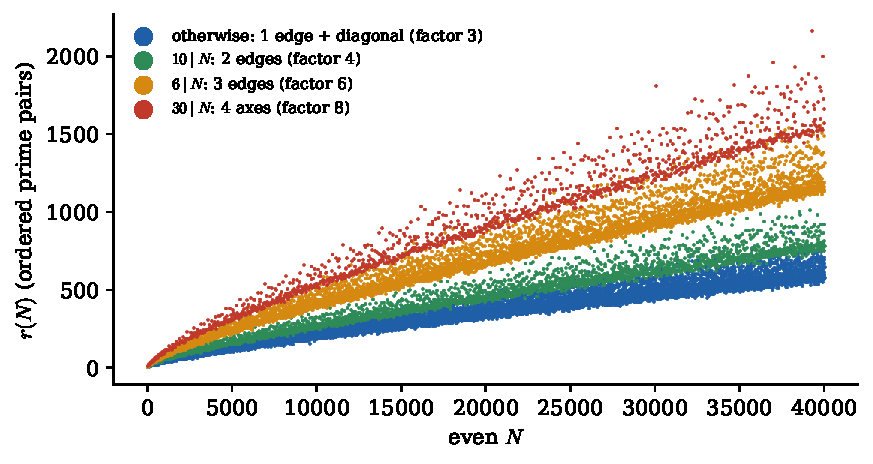
\includegraphics[width=0.66\linewidth]{figures/fig_goldbach.pdf}
\caption{The Goldbach comet $r(N)$ for even $N\le40000$, coloured by the four
classes of the local factor at $30$ (\cref{thm:B1}). The bands are ordered by
the factors $3,4,6,8$; further splitting within the bands comes from the primes
$7,11,\dots$ dividing $N$.}
\label{fig:goldbach}
\end{figure}

\subsection{Sophie Germain primes and Cunningham chains}
\begin{proposition}[\statS]\label{prop:sg}
If $p>5$ and $2p+1$ are both prime, then $p\equiv11,23,29\pmod{30}$, and the
map $p\mapsto2p+1$ sends these classes to $23,17,29$. Consequently, in a
Cunningham chain $p,2p+1,4p+3,\dots$ of length $\ge4$ with all members $>5$,
every member is $\equiv29\pmod{30}$, i.e.\ the whole chain sits on the single
vertex $A_1^-$ of the $16$-cell.
\end{proposition}
\begin{proof}
$2r+1$ is a unit modulo $30$ exactly for $r\in\{11,23,29\}$ among the units.
Starting in $11$ the chain runs $11\to23\to17$ and stops (as $17$ is not
admissible), starting in $23$ it runs $23\to17$; only $29\mapsto29$ can be
iterated.
\end{proof}
Under the Bateman--Horn conjecture \cite{BatemanHorn} the number of Sophie
Germain primes up to $x$ is $\sim2C_2\,x/(\log x\log2x)$ \statH; infinitude is
open \statO. Example: the chain $89,179,359,719,1439,2879$ lies on $A_1^-$.

\subsection{Chen and Lemoine}
Lemoine's conjecture (every odd $N\ge7$ is $p+2q$ with primes $p,q$) has the
same local structure as Goldbach: the number of $(a,b)\in U(M_k)^2$ with
$a+2b\equiv N$ is again $\prod_{3\le p\le p_k}N_p(N)$ \statS, because
$b\mapsto2b$ is a bijection of $U(p)$. Chen's theorem is the strongest
classical anchor for both families; the lifting problems are open \statO.

\subsection{Prime races}
By Dirichlet's theorem and the prime number theorem in progressions, the eight
vertices of the $16$-cell are asymptotically equally occupied
\cite{Dirichlet}: up to $10^8$ each class contains about $720\,000$ primes
\statN. Finer effects are not equidistributed. Chebyshev's bias (non-residue
classes lead most of the time) is explained, under GRH and a linear
independence hypothesis, by Rubinstein--Sarnak \cite{RubSarnak}. Consecutive
primes avoid repeating their residue class (Lemke Oliver--Soundararajan
\cite{LOS}): up to $10^8$ the proportion of consecutive primes in the
\emph{same} class modulo $30$ is $0.0443$, against $1/8=0.125$ for
independent classes \statN. In the geometry, a step to the same vertex is the
rarest step; the explanation is analytic (second-order terms of the
Hardy--Littlewood conjecture), not geometric.

% =====================================================================
\section{Applications III: tuples and polynomials}\label{sec:tuples}

\begin{plainwords}
The same recipe works for longer patterns: prime triplets such as
$(p,p+2,p+6)$, quadruplets $(p,p+2,p+6,p+8)$, and values of polynomials such
as $n^2+1$. In each case the polytope picks out the admissible corners (for
$n^2+1$ they form a single tetrahedral cell of the $16$-cell), the exact count
converges to the Hardy--Littlewood constant, and the numbers up to $10^8$
match the prediction to within a few parts per thousand. For long arithmetic
progressions of primes the situation is different: here the existence problem
has been solved (Green--Tao), and the geometry shows why such progressions must
sit on a single corner.
\end{plainwords}

\subsection{Hardy--Littlewood constellations}
For an admissible $H$ with $m$ elements, \cref{prop:crt,prop:singular} give the
exact count and the constant. The Hardy--Littlewood conjecture
\cite{HL} predicts $\#\{p\le x:p+h\text{ prime }\forall h\in H\}\sim\mathfrak
S(H)\Li_m(x)$; it is open for every $m\ge2$ \statO. The Maynard--Tao method
\cite{Maynard} shows: for every $m$, every sufficiently large admissible pattern
contains $m$ elements that are simultaneously prime for infinitely many
translates.
\begin{observation}[\statN]
Up to $x=10^8$: triplets $\{0,2,6\}$: $55\,600$; $\{0,4,6\}$: $55\,556$;
prediction $\mathfrak S\,\Li_3(x)=55\,491$ with $\mathfrak S=2.8582$.
Quadruplets $\{0,2,6,8\}$: $4\,768$; prediction $4\,735$ with
$\mathfrak S=4.1512$.
\end{observation}
Exact counts $N_k(H)$ for these patterns at $k=2,\dots,7$ are in
\cref{app:tables}; see \cite{K-hl}.

\subsection{Landau \texorpdfstring{$n^2+1$}{n2+1} and Bunyakovsky--Schinzel}
\begin{theorem}[\statS]\label{thm:landau}
Every prime of the form $n^2+1$ larger than $5$ is congruent to $1,7,11$ or
$17$ modulo $30$. These four classes form one tetrahedral cell of the $16$-cell
(one vertex on each axis: $A_1^+,A_2^+,A_3^+,A_4^-$).
\end{theorem}
\begin{proof}
$n$ must be even, and running through the even residues modulo $30$ gives
$n^2+1\bmod30\in\{1,5,7,11,17,25\}$; the classes $5$ and $25$ are excluded.
The four remaining classes lie on four different axes, hence span a cell.
\end{proof}
\begin{conditional}[Hardy--Littlewood conjecture F \cite{HL}, Bateman--Horn \cite{BatemanHorn}]
$\#\{n\le x:n^2+1\text{ prime}\}\sim\frac C2\li(x)$ with
$C=\prod_{p>2}\bigl(1-\frac{(-1/p)}{p-1}\bigr)=1.37281\ldots$
\end{conditional}
\begin{observation}[\statN]
For $x=10^3,10^4,10^5,2\cdot10^5$ the counts are $112$, $841$, $6\,656$,
$12\,391$; the predictions are $121$, $855$, $6\,609$, $12\,379$.
\end{observation}
\paragraph{Classical anchor.} $n^2+1$ has at most two prime factors for
infinitely many $n$ (Iwaniec \cite{Iwaniec}). Landau's problem is open \statO.
The cell of \cref{thm:landau} is the geometric carrier; the constant $C$ is
the limit of its truncated singular series, where the Legendre symbol $(-1/p)$
(\cref{prop:languages}(3)) decides whether $p$ removes two or zero residues.

\subsection{Primes in arithmetic progression (Green--Tao)}
\begin{proposition}[\statS]\label{prop:ap}
Let $a,a+d,\dots,a+(\ell-1)d$ be primes, all $>\ell$. Then every prime
$q\le\ell$ divides $d$. Hence, if $p_k\le\ell$, all terms are congruent modulo
$M_k$: the whole progression sits on a single vertex of
$\beta_{\varphi(M_k)/2}$.
\end{proposition}
\begin{proof}
If $q\nmid d$, the $\ell\ge q$ terms cover all residues modulo $q$, so one term
is divisible by $q$; being $>\ell\ge q$, it is not prime.
\end{proof}
Green and Tao proved that the primes contain arbitrarily long arithmetic
progressions \cite{GreenTao}. In the language of the cascade: the
``single-vertex'' configurations of every length lift \statS. This is one of
the few classical lifting problems that is solved, and it shows that the
lifting step requires analytic input of a completely different kind
(higher-order Fourier analysis, transference) from the local counts that the
geometry provides.

% =====================================================================
\section{Applications IV: exponential families and self-correlation}\label{sec:exp}

\begin{plainwords}
Some famous prime families grow exponentially: Mersenne numbers $2^p-1$,
Fermat numbers $2^{2^n}+1$, repunits $11\ldots1$. For them the polytope does
something simple and exact: it tells us on which corner of the $16$-cell the
members must sit (Mersenne primes on two corners, repunit primes on two
others). The expected number of such primes grows only like a logarithm. A
second group (Wieferich, Wilson, Wolstenholme primes) is defined by a
condition modulo $p^2$ at the prime itself; such conditions are invisible to
the polytope, which only sees remainders modulo small fixed primes. Finally,
there are numbers $k$ for which $k\cdot2^n+1$ is \emph{never} prime; here the
local obstruction is total, and the polytope sees it completely.
\end{plainwords}

\subsection{AP-factor families}
\begin{proposition}[\statS]\label{prop:mersenne}
Let $p\ge5$ be prime. Then $2^p-1\equiv1\pmod{30}$ if $p\equiv1\pmod4$ and
$2^p-1\equiv7\pmod{30}$ if $p\equiv3\pmod4$. Every prime factor $q$ of $2^p-1$
satisfies $q\equiv1\pmod{2p}$ and $q\equiv\pm1\pmod8$.
\end{proposition}
\begin{proof}
$2^p\equiv2\pmod3$ for odd $p$, and $2^p\bmod5$ is $2$ or $3$ according as
$p\equiv1$ or $3\pmod4$; combine with oddness. The divisor statement is
classical: the order of $2$ modulo $q$ is $p$, so $p\mid q-1$; and $2$ is a
quadratic residue modulo $q$ since $2\equiv(2^{(p+1)/2})^2$ \cite{HardyWright}.
\end{proof}
So Mersenne primes beyond $7$ occupy only the vertices $A_1^+$ and $A_2^+$.
The Lenstra--Pomerance--Wagstaff heuristic predicts
$\#\{p\le x:2^p-1\text{ prime}\}\sim(e^\gamma/\log2)\log x$ \statH\
\cite{Wagstaff}.

\begin{proposition}[\statS]\label{prop:repunit}
Let $R_n=(10^n-1)/9$ be the repunit with $n>3$ prime. Then
$R_n\equiv1\pmod{30}$ if $n\equiv1\pmod3$ and $R_n\equiv11\pmod{30}$ if
$n\equiv2\pmod3$.
\end{proposition}
\begin{proof}
$R_n$ is odd and $\equiv1\pmod5$; modulo $3$ it is congruent to its digit sum
$n$.
\end{proof}
Cullen ($n2^n+1$), Woodall ($n2^n-1$) and Proth-type families
($k2^n+1$ for fixed $k$) are handled in the same way: a half-axis or a small
set of half-axes is forced by the exponent modulo small numbers, and the
heuristic count grows logarithmically \statH\ \cite{K-atlas}.

\subsection{Sierpi\'{n}ski and Riesel}
For $k=78557$ every number $k\cdot2^n+1$ is divisible by one of
$3,5,7,13,19,37,73$ (Selfridge, see \cite{Sierpinski}); for $k=509203$ every
$k\cdot2^n-1$ is divisible by one of $3,5,7,13,17,241$ (Riesel
\cite{Riesel}) \statS. In the language of the cascade, a covering
congruence means that for each exponent $n$ the number lands on a
\emph{non-unit} residue at some fixed finite level: the local obstruction is
complete, and the count of \cref{prop:crt} is zero. These families are the
boundary case of the growth law: the logarithmic heuristic has constant~$0$.

\subsection{Self-correlation families}
Wieferich primes ($2^{p-1}\equiv1\bmod p^2$; known: $1093$, $3511$), Wilson
primes ($(p-1)!\equiv-1\bmod p^2$; known: $5$, $13$, $563$),
Wall--Sun--Sun primes (none known) and Wolstenholme primes
($\binom{2p-1}{p-1}\equiv1\bmod p^4$; known: $16843$, $2124679$) are defined by
a condition modulo a power of the prime itself \statN. If such a condition is
satisfied with probability $1/p$, the expected number up to $x$ is
$\sum_{p\le x}1/p\sim\log\log x$ \statH. The condition is not a residue
condition modulo the fixed small primes of the cascade; the geometry is
blind to these families \statG, which is an honest limit of the method.

\subsection{Boundary objects and fractal classification}
Fibonacci and Lucas primes reduce to progressions through the rank of
apparition; Carmichael numbers (Korselt's criterion) are composites that pass
the Fermat test, and there are infinitely many \cite{AGP}. In \cite{K-atlas}
prime families are also compared by the finite-scale box-counting dimension of
their logarithmic embedding $p\mapsto\log p/\log p_{\max}\in[0,1]$: positive
density families sit near $0.87$, constellations lower, and exponential
families tend to $0$ (a ``log-ladder'') \statN. This is a diagnostic, not a
topological invariant (every countable set has Hausdorff dimension $0$).

% =====================================================================
\section{Collatz as a test case for non-locality}\label{sec:collatz}

\begin{plainwords}
The Collatz rule ($n\mapsto3n+1$ for odd $n$, $n\mapsto n/2$ for even $n$) is
not a question about primes, but it is a perfect test of the method. Its
statistics look exactly like a random process with a downward drift, and all
local information (remainders modulo small numbers) is evenly spread. Yet
nobody can prove that every starting value reaches $1$. The case shows in
pure form what the whole paper finds: local data can explain averages, but not
the fate of every single number.
\end{plainwords}

\paragraph{Cycle equation \statS.} Write an orbit through odd numbers
$x_1,\dots,x_n$ with $x_{i+1}=(3x_i+1)/2^{a_i}$. A cycle of length $n$ with
$m=\sum a_i$ halvings satisfies
$2^m=\prod_{i=1}^n(3+1/x_i)$, so $m/n$ is close to $\log_23$ for cycles with
large elements; this is the starting point of all known lower bounds on
cycle lengths \cite{Lagarias}.

\paragraph{Drift \statH.} If the number $a_i=v_2(3x_i+1)$ of halvings after
an odd step behaves like a geometric random variable with mean $2$, the mean
change of $\log_2x$ per odd step is $\log_23-2\approx-0.415<0$. For the
generalised map $n\mapsto pn+1$ the drift is $\log_2p-2$, negative only for
$p=3$ among odd primes \cite{K-collatz}.

\paragraph{Numerics \statN.} The value $9232$ is the maximum of the trajectory
for exactly $1579$ starting values (all of them below $9232$, so the count is
the same for $N=10^4,10^5,10^6$). The detrended log-trajectories show a
spectral crossover near period six, twice the mean distance between odd steps
\cite{K-collatz}.

\paragraph{Anchor and limit.} Tao proved that almost all orbits attain almost
bounded values \cite{Tao}; the conjecture is open \statO. The map
$n\mapsto3n+1$ sends every odd $n$ to the class $1\bmod3$, so it does not
preserve the unit structure of the cascade; there is no orbit-minimum
formulation. Collatz is included as a control case for non-locality
(\cref{sec:closure}).

% =====================================================================
\section{Spectral reflection}\label{sec:spectral}

\begin{plainwords}
The constants that appeared above (the twin constant $C_2$, Artin's constant,
the Landau--Ramanujan constant, the Mertens constant) can all be written as
the ``determinant'' of a very simple operator: one number per prime, placed on
a diagonal. This repackaging is exact and elementary. Its use is that it
shows which constants belong together. In particular the split of the primes
by their remainder modulo~$4$ appears three times in this paper (sums of two
squares, the Legendre sign of the flips, and the Landau--Ramanujan constant),
and the operator picture makes it one and the same projection.
\end{plainwords}

Let $D$ be the diagonal operator on $\ell^2(\{\text{primes}\})$ and $t_p$ its
entries. If $\sum_p|t_p|<\infty$, then $\exp(\operatorname{tr}D)=\prod_pe^{t_p}$
is a Fredholm-type determinant \statS. With
\begin{center}
\begin{tabular}{lll}\toprule
constant & $e^{t_p}$ & value\\\midrule
$C_2$ (twins) & $1-(p-1)^{-2}$, $p\ge3$ & $0.6601618\ldots$\\
Artin $A$ & $1-\frac1{p(p-1)}$ & $0.3739558\ldots$\\
$e^{M-\gamma}$ (Mertens) & $(1-\frac1p)e^{1/p}$ & $e^{-0.3157\ldots}$\\
$\sqrt2\,K$ (Landau--Ramanujan) & $(1-p^{-2})^{-1/2}$ for $p\equiv3\bmod4$, else $1$ & $\sqrt2\cdot0.7642236\ldots$\\\bottomrule
\end{tabular}
\end{center}
the four constants are exponentials of traces \cite{K-c2,K-trace}. The last
line uses the projector $P_3$ onto the primes $p\equiv3\pmod4$; the same
projector selects the primes whose sign flip changes the quadratic character
(\cref{prop:languages}(3)) and the primes that are not sums of two squares.
This is a bookkeeping identity \statG; it carries no spectral information
about zeros of $\zeta$.

% =====================================================================
\section{Two notions of closure and the limit of the method}\label{sec:closure}

\begin{plainwords}
Two different things can be called ``closing'' a problem about primes. The
geometric closure is complete: for every pattern we know exactly which
corners are allowed and how many there are, at every level, and how this
converges to the predicted constant. The analytic closure is the statement
that the allowed corners are really filled with primes, again and again.
Only the second one decides the famous conjectures, and it does not follow
from the first. The reason is a kind of non-locality: whether a number is a
prime depends on all of its potential divisors at once, not on a fixed finite
set of them; the orbit-minimum property is already global on each hypercube
(\cref{obs:nonlocal}).
\end{plainwords}

\paragraph{Geometric closure \statS.} For every admissible pattern the exact
count $N_k(H)$, its truncated singular series and the limit $\mathfrak S(H)$
are determined (\cref{prop:crt,prop:singular}); the same holds for the
Goldbach and Lemoine counts (\cref{thm:goldbach}) and for the polynomial case
$n^2+1$ (\cref{thm:landau}).

\paragraph{Analytic closure.} The step from local counts to primes requires
estimates for primes in short intervals or progressions beyond what sieve
methods give. A classical reason is the parity barrier of the Selberg sieve:
local information cannot distinguish numbers with an even from numbers with
an odd number of prime factors \cite{FriedlanderIwaniec}. This is why Chen's
theorems stop at $P_2$, and why the cascade, which consists of local
information only, cannot replace the analytic step.

\begin{table}[!htbp]
\centering\small
\caption{Status of the lifting problem in the language of the cascade.}
\label{tab:lifting}
\begin{tabular}{p{5.4cm}p{2.2cm}p{6.2cm}}\toprule
configuration & lifting status & strongest classical result\\\midrule
single vertex (APs mod $q$) & solved \statS & Dirichlet; PNT in progressions\\
single vertex, long APs & solved \statS & Green--Tao \cite{GreenTao}\\
some edge of length $\le246$ & solved \statS & Maynard, Polymath \cite{Maynard,Polymath}\\
translated antipode, 3 summands & solved \statS & Helfgott \cite{Helfgott}\\
twin edge $\{0,2\}$ & open \statO & Chen \cite{Chen}\\
Polignac edges $\{0,d\}$ & open \statO & bounded gaps\\
antipode $p+q=N$ (Goldbach) & open \statO & Chen; Montgomery--Vaughan \cite{MV}\\
cell $n^2+1$ & open \statO & Iwaniec \cite{Iwaniec}\\
windows (Legendre, Brocard) & open \statO & Baker--Harman--Pintz \cite{BHP}\\
half-axis $A_4^-$ (Fermat) & open \statO & heuristic finiteness\\
Collatz (control case) & open \statO & Tao \cite{Tao}\\\bottomrule
\end{tabular}
\end{table}

% =====================================================================
\section{Outlook}\label{sec:outlook}
Three directions of the series lie outside the scope of this synthesis and are
only mentioned. (i) The antipodal involution defines a ``half-line'' on which
several classical halvings coincide \cite{K-halfline}. (ii) Minima of an
amplitude derived from the matchstick machine on the line $\Re s=\frac12$
show a numerical coincidence with zeros of $\zeta$ \cite{K-zeta}; this is a
numerical observation, not an argument for the Riemann hypothesis. (iii) A
generator model of primality from geometric principles is developed in
\cite{K-generator}. The tower of fields above the cascade and the
interpretative strand of the series are treated separately.

% =====================================================================
\appendix
\section{Proofs in full}\label{app:proofs}
All proofs of \cref{sec:16cell,sec:cascade,sec:four,sec:scheme} are complete
in the text. We collect here the two points where a reader may want more
detail.

\paragraph{A.1 Lemma~\ref{lem:threshold}, the finite part.} The induction step
needs $p_{k+1}\ge17$, i.e.\ $k\ge6$, and the base case
$4M_6=120120\ge83521=17^4$. For $k\le5$ the inequality fails, as listed. Hence
the equivalence.

\paragraph{A.2 Orbit partners at $k=5$.} Using \cref{prop:orbitcrit}, $n$ is
not an orbit minimum iff there is a unit $z<n$ with $z^2\equiv n^2\pmod{2310}$.
For $n=97,101,103,107$ the smallest such $z$ is $13,31,37,47$, and in each
case $n^2-z^2=9240=4M_5$, the smallest value allowed by \cref{lem:key}.
For the primes $n\le96$ no such $z$ exists, because $n^2<4M_5=9240$.

\paragraph{A.3 Spectrum of $T$.} Fix an orbit $O$ and $a\in O$. The map
$g\mapsto ga$ identifies $O$ with $G_k$, and functions on $O$ with the regular
representation. The characters $\chi_S(g)=\prod_{j\in S}\epsilon_j(g)$ form an
eigenbasis of every $U_j$, with $U_j\chi_S=\pm\chi_S$ according as $j\notin S$
or $j\in S$. Summing gives the eigenvalue $(1+(k-1-|S|)-|S|)/k$.

\section{Reference code}\label{app:code}
The following Python code (requires \texttt{sympy}) computes orbit minima via
the orbit criterion and checks \cref{thm:completeness,prop:sharp,cor:count}
for $k=3,\dots,7$; it also reproduces the incidence counts of
\cref{prop:sums} and the local minima of \cref{obs:nonlocal}.
\begin{lstlisting}
from sympy import primorial, prime, isprime, primerange
from math import gcd
from itertools import combinations

def orbit_minima(k):
    """B_k: smallest representative of every square class of U(M_k)."""
    M = int(primorial(k)); best = {}
    for y in range(1, M):
        if gcd(y, M) == 1:
            s = y * y % M
            if s not in best:      # y increases, so the first hit is the minimum
                best[s] = y
    return M, sorted(best.values())

def check(k):
    M, B = orbit_minima(k); pk, pn = prime(k), prime(k + 1)
    phi = 1
    for i in range(1, k + 1): phi *= prime(i) - 1
    low  = [b for b in B if 1 < b <= pn * pn]
    pred = list(primerange(pk + 1, pn * pn)) + [pn * pn]
    comp = [b for b in B if b > 1 and not isprime(b)]
    return dict(k=k, orbits=len(B), formula=phi // 2**(k - 1),
                completeness=(low == pred), smallest_composite=min(comp) if comp else None,
                p_next=min(b for b in B if b > 1))

def local_minima(k):
    """Units smaller than all single-flip neighbours sigma_j(a)."""
    M = int(primorial(k)); E = []
    for j in range(2, k + 1):
        p = prime(j); m = M // p
        E.append(next(e for e in range(1, M) if e % p == p - 1 and e % m == 1 % m))
    return sum(1 for a in range(1, M) if gcd(a, M) == 1
               and all(a < e * a % M for e in E))

def incidences():
    U = [a for a in range(1, 30) if gcd(a, 30) == 1]
    face = lambda S: all((a + b) % 30 for a, b in combinations(S, 2))
    edges = [S for S in combinations(U, 2) if face(S)]
    facets = [S for S in combinations(U, 3) if face(S)]
    cells = [S for S in combinations(U, 4) if face(S)]
    return len(edges), len(facets), len(cells)   # (24, 32, 16)

if __name__ == "__main__":
    for k in range(3, 8):
        print(check(k), local_minima(k) if k <= 6 else "")
    print(incidences())
\end{lstlisting}

\section{Tables}\label{app:tables}
\begin{table}[H]
\centering\small
\caption{Exact counts $N_k(H)$ of \cref{prop:crt} for the twin pattern
$\{0,2\}$, the Polignac pattern $\{0,6\}$, the triplet $\{0,2,6\}$ and the
quadruplet $\{0,2,6,8\}$.}
\label{tab:counts}
\begin{tabular}{rrrrrrr}\toprule
$k$ & $M_k$ & $\varphi(M_k)$ & $\{0,2\}$ & $\{0,6\}$ & $\{0,2,6\}$ & $\{0,2,6,8\}$\\\midrule
2 & 6 & 2 & 1 & 2 & 1 & 1\\
3 & 30 & 8 & 3 & 6 & 2 & 1\\
4 & 210 & 48 & 15 & 30 & 8 & 3\\
5 & 2\,310 & 480 & 135 & 270 & 64 & 21\\
6 & 30\,030 & 5\,760 & 1\,485 & 2\,970 & 640 & 189\\
7 & 510\,510 & 92\,160 & 22\,275 & 44\,550 & 8\,960 & 2\,457\\\bottomrule
\end{tabular}
\end{table}

\begin{table}[H]
\centering\small
\caption{Addresses $(k,A_i,\pm,s)$ of the primes $7\le p\le113$
(\cref{def:address}).}
\label{tab:addresses}
\begin{tabular}{rl@{\qquad}rl@{\qquad}rl@{\qquad}rl}\toprule
$p$ & address & $p$ & address & $p$ & address & $p$ & address\\\midrule
7 & $(3,A_2,+,0)$ & 31 & $(4,A_1,+,1)$ & 59 & $(4,A_1,-,1)$ & 89 & $(4,A_1,-,2)$\\
11 & $(3,A_3,+,0)$ & 37 & $(4,A_2,+,0)$ & 61 & $(4,A_1,+,2)$ & 97 & $(4,A_2,+,2)$\\
13 & $(3,A_4,+,0)$ & 41 & $(4,A_3,+,1)$ & 67 & $(4,A_2,+,1)$ & 101 & $(4,A_3,+,3)$\\
17 & $(3,A_4,-,0)$ & 43 & $(4,A_4,+,1)$ & 71 & $(4,A_3,+,2)$ & 103 & $(4,A_4,+,3)$\\
19 & $(3,A_3,-,0)$ & 47 & $(4,A_4,-,1)$ & 73 & $(4,A_4,+,2)$ & 107 & $(4,A_4,-,2)$\\
23 & $(3,A_2,-,0)$ & 53 & $(4,A_2,-,1)$ & 79 & $(4,A_3,-,1)$ & 109 & $(4,A_3,-,2)$\\
29 & $(3,A_1,-,0)$ &    &               & 83 & $(4,A_2,-,2)$ & 113 & $(4,A_2,-,3)$\\\bottomrule
\end{tabular}
\end{table}

\section{Glossary for non-specialists}\label{app:glossary}
\begin{description}[leftmargin=0pt,itemsep=2pt,font=\normalfont\bfseries]
\item[Unit modulo $M$.] A remainder $a$ with $\gcd(a,M)=1$; only units can be
remainders of primes not dividing $M$.
\item[Primorial $M_k$.] The product of the first $k$ primes: $2,6,30,210,2310,\dots$
\item[Cross-polytope $\beta_d$.] The $d$-dimensional generalisation of the
octahedron: $2d$ corners $\pm e_i$, every pair of non-opposite corners joined.
The $16$-cell is $\beta_4$.
\item[Axis, half-axis.] A pair $\{a,M-a\}$ of mirror remainders; each of its two
members is a half-axis.
\item[Sign flip $\sigma_j$.] Changing the sign of a remainder modulo one prime
$p_j$ only.
\item[Orbit, orbit minimum.] All remainders reachable by sign flips; the
smallest of them.
\item[Hypercube $Q_d$.] The $d$-dimensional cube; each orbit is one.
\item[Admissible pattern.] A set of shifts $H$ that does not cover all
remainders modulo any prime; otherwise one member is always divisible by that
prime.
\item[Singular series $\mathfrak S(H)$.] The product of local correction factors
in the Hardy--Littlewood prediction; here the limit of exact vertex counts.
\item[Lifting problem.] Showing that admissible configurations are actually
realised by primes infinitely often.
\item[Status marks.] \statS\ proved, \statG\ exact reformulation, \statN\
numerical, \statH\ heuristic, \statO\ open.
\end{description}

% =====================================================================
\section*{Data and code availability}
\addcontentsline{toc}{section}{Data and code availability}
The reference code is reproduced in \cref{app:code}. All numerical values in
this paper were recomputed with an independent Python script (NumPy sieve up
to $10^8$). This script, its complete output and the script that generates all
figures are provided as supplementary material with this preprint
(files \texttt{numerics\_check.py}, \texttt{numerics\_output.txt} and
\texttt{figs.py}; the check runs in under one minute).
The earlier papers of the series are openly available under the DOIs listed in
the references.

\section*{Funding}
\addcontentsline{toc}{section}{Funding}
This research received no external funding.

\section*{Conflicts of interest}
\addcontentsline{toc}{section}{Conflicts of interest}
The author declares no conflicts of interest.

\section*{Acknowledgements}
\addcontentsline{toc}{section}{Acknowledgements}
The author thanks the readers of the earlier papers of the series for their
questions. Computations used Python with \texttt{sympy}, \texttt{numpy} and
\texttt{matplotlib}.

\begin{thebibliography}{99}\small
\setlength{\itemsep}{1pt}
% --- classical literature ---
\bibitem{AGP} W.~R.~Alford, A.~Granville, C.~Pomerance, There are infinitely many
Carmichael numbers, \emph{Ann. of Math.} 139 (1994) 703--722.
\bibitem{BHP} R.~C.~Baker, G.~Harman, J.~Pintz, The difference between
consecutive primes, II, \emph{Proc. London Math. Soc.} 83 (2001) 532--562.
\bibitem{BatemanHorn} P.~T.~Bateman, R.~A.~Horn, A heuristic asymptotic
formula concerning the distribution of prime numbers, \emph{Math. Comp.} 16
(1962) 363--367.
\bibitem{Chen} J.-R.~Chen, On the representation of a larger even integer as
the sum of a prime and the product of at most two primes, \emph{Sci. Sinica}
16 (1973) 157--176.
\bibitem{Coxeter} H.~S.~M.~Coxeter, \emph{Regular Polytopes}, 3rd ed., Dover,
New York, 1973.
\bibitem{Dirichlet} P.~G.~L.~Dirichlet, Beweis des Satzes, dass jede
unbegrenzte arithmetische Progression \dots\ unendlich viele Primzahlen
enthält, \emph{Abh. Königl. Preuss. Akad. Wiss.} (1837) 45--81.
\bibitem{Erdos32} P.~Erd\H{o}s, Beweis eines Satzes von Tschebyschef, \emph{Acta
Litt. Sci. Szeged} 5 (1932) 194--198.
\bibitem{FriedlanderIwaniec} J.~Friedlander, H.~Iwaniec, \emph{Opera de
Cribro}, AMS Colloquium Publications 57, 2010.
\bibitem{GreenTao} B.~Green, T.~Tao, The primes contain arbitrarily long
arithmetic progressions, \emph{Ann. of Math.} 167 (2008) 481--547.
\bibitem{HL} G.~H.~Hardy, J.~E.~Littlewood, Some problems of `Partitio
numerorum'; III: On the expression of a number as a sum of primes, \emph{Acta
Math.} 44 (1923) 1--70.
\bibitem{HardyWright} G.~H.~Hardy, E.~M.~Wright, \emph{An Introduction to the
Theory of Numbers}, 6th ed., Oxford University Press, 2008.
\bibitem{Helfgott} H.~A.~Helfgott, The ternary Goldbach problem,
arXiv:1501.05438 (2015).
\bibitem{Ingham} A.~E.~Ingham, On the difference between consecutive primes,
\emph{Quart. J. Math. Oxford} 8 (1937) 255--266.
\bibitem{Iwaniec} H.~Iwaniec, Almost-primes represented by quadratic
polynomials, \emph{Invent. Math.} 47 (1978) 171--188.
\bibitem{Lagarias} J.~C.~Lagarias (ed.), \emph{The Ultimate Challenge: The
$3x+1$ Problem}, American Mathematical Society, 2010.
\bibitem{LOS} R.~J.~Lemke Oliver, K.~Soundararajan, Unexpected biases in the
distribution of consecutive primes, \emph{Proc. Natl. Acad. Sci. USA} 113
(2016) E4446--E4454.
\bibitem{Maynard} J.~Maynard, Small gaps between primes, \emph{Ann. of Math.}
181 (2015) 383--413.
\bibitem{Mertens} F.~Mertens, Ein Beitrag zur analytischen Zahlentheorie,
\emph{J. Reine Angew. Math.} 78 (1874) 46--62.
\bibitem{MV} H.~L.~Montgomery, R.~C.~Vaughan, The exceptional set in
Goldbach's problem, \emph{Acta Arith.} 27 (1975) 353--370.
\bibitem{Nicolas71} J.-L.~Nicolas, Répartition des nombres hautement composés
de Ramanujan, \emph{Canad. J. Math.} 23 (1971) 116--130.
\bibitem{Nicolas83} J.-L.~Nicolas, Petites valeurs de la fonction d'Euler,
\emph{J. Number Theory} 17 (1983) 375--388.
\bibitem{OeSilva} T.~Oliveira e Silva, S.~Herzog, S.~Pardi, Empirical
verification of the even Goldbach conjecture and computation of prime gaps up
to $4\cdot10^{18}$, \emph{Math. Comp.} 83 (2014) 2033--2060.
\bibitem{Polymath} D.~H.~J.~Polymath, Variants of the Selberg sieve, and
bounded intervals containing many primes, \emph{Res. Math. Sci.} 1 (2014),
Art.~12.
\bibitem{Ramanujan} S.~Ramanujan, Highly composite numbers, \emph{Proc. London
Math. Soc.} (2) 14 (1915) 347--409.
\bibitem{Riesel} H.~Riesel, Några stora primtal, \emph{Elementa} 39 (1956)
258--260.
\bibitem{RubSarnak} M.~Rubinstein, P.~Sarnak, Chebyshev's bias,
\emph{Experiment. Math.} 3 (1994) 173--197.
\bibitem{Sierpinski} W.~Sierpi\'{n}ski, Sur un problème concernant les nombres
$k\cdot2^n+1$, \emph{Elem. Math.} 15 (1960) 73--74.
\bibitem{Tao} T.~Tao, Almost all orbits of the Collatz map attain almost
bounded values, \emph{Forum Math. Pi} 10 (2022) e12.
\bibitem{Wagstaff} S.~S.~Wagstaff, Divisors of Mersenne numbers, \emph{Math.
Comp.} 40 (1983) 385--397.
\bibitem{Zhang} Y.~Zhang, Bounded gaps between primes, \emph{Ann. of Math.}
179 (2014) 1121--1174.
% --- series "Geometry of Reality" (T. Krause, 2026, Zenodo) ---
\bibitem{K-matchstick} T.~Krause, The matchstick game and its information: a
geometric reading of Euler's product formula and Ramanujan's highly composite
numbers, Zenodo (2026), \href{https://doi.org/10.5281/zenodo.20525797}{doi:10.5281/zenodo.20525797}.
\bibitem{K-collatz} T.~Krause, Spectral cross-over and filter mechanics in
Collatz trajectories, Zenodo (2026),
\href{https://doi.org/10.5281/zenodo.20527222}{doi:10.5281/zenodo.20527222}.
\bibitem{K-nicolas} T.~Krause, The constant $\log30/\log16$ in Nicolas: a
didactic derivation, Zenodo (2026),
\href{https://doi.org/10.5281/zenodo.20556204}{doi:10.5281/zenodo.20556204}.
\bibitem{K-triangle} T.~Krause, The prime number geometry via triangle game and
square atlas, Zenodo (2026),
\href{https://doi.org/10.5281/zenodo.20600998}{doi:10.5281/zenodo.20600998}.
\bibitem{K-16cell} T.~Krause, The geometry of primes: the 16-cell as the seat
of the eight coprime classes modulo 30, Zenodo (2026),
\href{https://doi.org/10.5281/zenodo.20607940}{doi:10.5281/zenodo.20607940}.
\bibitem{K-recursive} T.~Krause, A geometric recursion formula for prime
numbers, Zenodo (2026),
\href{https://doi.org/10.5281/zenodo.20663415}{doi:10.5281/zenodo.20663415}.
\bibitem{K-tool} T.~Krause, A geometric algorithm enumerating all primes in
$(p_k,p_k^2]$ in order via orbit minima, Zenodo (2026),
\href{https://doi.org/10.5281/zenodo.20687230}{doi:10.5281/zenodo.20687230}.
\bibitem{K-devil} T.~Krause, What the Devil's Game teaches us about the prime
machine, Zenodo (2026),
\href{https://doi.org/10.5281/zenodo.20712948}{doi:10.5281/zenodo.20712948}.
\bibitem{K-bertrand} T.~Krause, Bertrand's postulate as a Pascal-dome balance,
Zenodo (2026),
\href{https://doi.org/10.5281/zenodo.20727562}{doi:10.5281/zenodo.20727562}.
\bibitem{K-goldbach} T.~Krause, Goldbach as a cross-polytope antipode, Zenodo
(2026), \href{https://doi.org/10.5281/zenodo.20757759}{doi:10.5281/zenodo.20757759}.
\bibitem{K-hl} T.~Krause, The Hardy--Littlewood prime constellation conjecture
as cross-polytope translation geometry, Zenodo (2026),
\href{https://doi.org/10.5281/zenodo.21009668}{doi:10.5281/zenodo.21009668}.
\bibitem{K-twin} T.~Krause, Twin primes as cross-polytope edge, Zenodo (2026),
\href{https://doi.org/10.5281/zenodo.21009722}{doi:10.5281/zenodo.21009722}.
\bibitem{K-fermat} T.~Krause, A geometric reading of the Fermat finiteness
conjecture via a deterministic prime machine, Zenodo (2026),
\href{https://doi.org/10.5281/zenodo.21023587}{doi:10.5281/zenodo.21023587}.
\bibitem{K-polignac} T.~Krause, The prime machine and Polignac's conjecture: a
translation axiom on the cross-polytope, Zenodo (2026),
\href{https://doi.org/10.5281/zenodo.21024323}{doi:10.5281/zenodo.21024323}.
\bibitem{K-goldbachJNT} T.~Krause, Goldbach's conjecture as an antipode axiom on
cross-polytopes, Zenodo (2026),
\href{https://doi.org/10.5281/zenodo.21025844}{doi:10.5281/zenodo.21025844}.
\bibitem{K-layers} T.~Krause, Four mathematical languages converge on the same
prime machine, Zenodo (2026),
\href{https://doi.org/10.5281/zenodo.21155848}{doi:10.5281/zenodo.21155848}.
\bibitem{K-foundations} T.~Krause, Foundations of the prime machine: a
geometric framework for primes via orbit minima of the primorial unit group,
Zenodo (2026),
\href{https://doi.org/10.5281/zenodo.21175687}{doi:10.5281/zenodo.21175687}.
\bibitem{K-zeta} T.~Krause, Minima of a matchstick-machine amplitude on
$\sigma=1/2$: a numerical coincidence with the Riemann zeros, Zenodo (2026),
\href{https://doi.org/10.5281/zenodo.21192794}{doi:10.5281/zenodo.21192794}.
\bibitem{K-halfline} T.~Krause, The half-line of a prime machine: four
coincident halves from one antipodal involution, Zenodo (2026),
\href{https://doi.org/10.5281/zenodo.21204098}{doi:10.5281/zenodo.21204098}.
\bibitem{K-book} T.~Krause, \emph{Geometrie der Wirklichkeit, Teil 2: Die
Primzahlmaschine}, Zenodo (2026),
\href{https://doi.org/10.5281/zenodo.21456979}{doi:10.5281/zenodo.21456979}.
\bibitem{K-atlas} T.~Krause, A complete structural atlas of prime families,
Zenodo (2026),
\href{https://doi.org/10.5281/zenodo.21639023}{doi:10.5281/zenodo.21639023}.
\bibitem{K-c2} T.~Krause, The twin prime constant $C_2$ as a
Mertens-renormalised edge density on a cross-polytope, Zenodo (2026),
\href{https://doi.org/10.5281/zenodo.21639474}{doi:10.5281/zenodo.21639474}.
\bibitem{K-trace} T.~Krause, Four trace identities on the diagonal prime
operator, Zenodo (2026),
\href{https://doi.org/10.5281/zenodo.21790341}{doi:10.5281/zenodo.21790341}.
\bibitem{K-generator} T.~Krause, A geometric origin of prime numbers: the
prime-property generator as a geometry-first model of primality, Zenodo
(2026), \href{https://doi.org/10.5281/zenodo.21902287}{doi:10.5281/zenodo.21902287}.
\end{thebibliography}

\end{document}
